%% abtex2-modelo-relatorio-tecnico.tex, v-1.7.1 laurocesar
%% Copyright 2012-2013 by abnTeX2 group at http://abntex2.googlecode.com/ 
%%
%% This work may be distributed and/or modified under the
%% conditions of the LaTeX Project Public License, either version 1.3
%% of this license or (at your option) any later version.
%% The latest version of this license is in
%%   http://www.latex-project.org/lppl.txt
%% and version 1.3 or later is part of all distributions of LaTeX
%% version 2005/12/01 or later.
%%
%% This work has the LPPL maintenance status `maintained'.
%% 
%% The Current Maintainer of this work is the abnTeX2 team, led
%% by Lauro César Araujo. Further information are available on 
%% http://abntex2.googlecode.com/
%%
%% This work consists of the files abntex2-modelo-relatorio-tecnico.tex,
%% abntex2-modelo-include-comandos and abntex2-modelo-references.bib
%%

% ------------------------------------------------------------------------
% ------------------------------------------------------------------------
% abnTeX2: Modelo de Relatório Técnico/Acadêmico em conformidade com 
% ABNT NBR 10719:2011 Informação e documentação - Relatório técnico e/ou
% científico - Apresentação
% ------------------------------------------------------------------------ 
% ------------------------------------------------------------------------

% Alterado por Rodrigo Campiolo para apresentação de relatórios na disciplina
% de Redes de Computadores II do Bacharelado em Ciência da Computação da UTFPR-CM.


\documentclass[
    % -- opções da classe memoir --
    12pt,				% tamanho da fonte
    %openright,			% capítulos começam em pág ímpar (insere página vazia caso preciso)
    oneside,   	        % para impressão em verso e anverso use twoside. Oposto a oneside
    a4paper,			% tamanho do papel. 
    % -- opções da classe abntex2 --
    %chapter=TITLE,		% títulos de capítulos convertidos em letras maiúsculas
    %section=TITLE,		% títulos de seções convertidos em letras maiúsculas
    %subsection=TITLE,	% títulos de subseções convertidos em letras maiúsculas
    %subsubsection=TITLE,% títulos de subsubseções convertidos em letras maiúsculas
    % -- opções do pacote babel --
    english,			% idioma adicional para hifenização
    french,				% idioma adicional para hifenização
    spanish,			% idioma adicional para hifenização
    brazil,				% o último idioma é o principal do documento
    ]{pacotes/abntex2}


% ---
% PACOTES
% ---

% ---
% Pacotes fundamentais 
% ---
\usepackage{cmap}				% Mapear caracteres especiais no PDF
\usepackage{lmodern}			% Usa a fonte Latin Modern
\usepackage[T1]{fontenc}		% Selecao de codigos de fonte.
\usepackage[utf8]{inputenc}		% Codificacao do documento (conversão automática dos acentos)
\usepackage{indentfirst}		% Indenta o primeiro parágrafo de cada seção.
\usepackage{color}				% Controle das cores
\usepackage{graphicx}			% Inclusão de gráficos
% ---

% ---
% Pacotes adicionais, usados no anexo do modelo de folha de identificação
% ---
\usepackage{multicol}
\usepackage{multirow}
% ---
    
% ---
% Pacotes adicionais, usados apenas no âmbito do Modelo Canônico do abnteX2
% ---
\usepackage{lipsum}				% para geração de dummy text
% ---

% ---
% Pacotes de citações
% ---
\usepackage[brazilian,hyperpageref]{backref}	 % Paginas com as citações na bibl
\usepackage[alf]{pacotes/abntex2cite}	% Citações padrão ABNT
\usepackage{comment}
% ---

% ---
% Meus pacotes
% ---
\usepackage{float}
\usepackage{listings}
\usepackage{color}

\definecolor{dkgreen}{rgb}{0,0.6,0}
\definecolor{gray}{rgb}{0.5,0.5,0.5}
\definecolor{mauve}{rgb}{0.58,0,0.82}

\lstset{frame=tb,
  language=C++,
  aboveskip=3mm,
  belowskip=3mm,
  showstringspaces=false,
  columns=flexible,
  basicstyle={\small\ttfamily},
  numbers=none,
  numberstyle=\tiny\color{gray},
  keywordstyle=\color{blue},
  commentstyle=\color{dkgreen},
  stringstyle=\color{mauve},
  breaklines=true,
  breakatwhitespace=true,
  tabsize=3,
  extendedchars=true,
  inputencoding=utf8x,
  texcl=true
}
% ---

% --- 
% CONFIGURAÇÕES DE PACOTES
% --- 

% ---
% Configurações do pacote backref
% Usado sem a opção hyperpageref de backref
\renewcommand{\backrefpagesname}{Citado na(s) página(s):~}
% Texto padrão antes do número das páginas
\renewcommand{\backref}{}
% Define os textos da citação
\renewcommand*{\backrefalt}[4]{
    \ifcase #1 %
        Nenhuma citação no texto.%
    \or
        Citado na página #2.%
    \else
        Citado #1 vezes nas páginas #2.%
    \fi}%
% ---

% ---
% Informações de dados para CAPA e FOLHA DE ROSTO
% ---
\titulo{Implementação do Sistema de Arquivos FAT32}
\autor{João Victor Briganti\\Luiz Gustavo Takeda\\Matheus Floriano Saito}
\local{Campo Mourão}
\data{Fevereiro / 2025}
\instituicao{%
  Universidade Tecnológica Federal do Paraná -- UTFPR
  \par
  Departa           mento Acadêmico de Computação -- DACOM
  \par
  Bacharelado em Ciência da Computação -- BCC
}
\tipotrabalho{Relatório técnico}
% O preambulo deve conter o tipo do trabalho, o objetivo, 
% o nome da instituição e a área de concentração 
\preambulo{Relatório técnico de atividade prática solicitado pelo professor Rodrigo Campiolo na disciplina de Sistemas Operacionais do Bacharelado em Ciência da Computação da Universidade Tecnológica Federal do Paraná.}
% ---

% ---
% Configurações de aparência do PDF final

% alterando o aspecto da cor azul
\definecolor{blue}{RGB}{41,5,195}

% informações do PDF
\makeatletter
\hypersetup{
        %pagebackref=true,
        pdftitle={\@title}, 
        pdfauthor={\@author},
        pdfsubject={\imprimirpreambulo},
        pdfcreator={LaTeX with abnTeX2},
        pdfkeywords={abnt}{latex}{abntex}{abntex2}{relatório técnico}, 
        colorlinks=true,       		% false: boxed links; true: colored links
        linkcolor=blue,          	% color of internal links
        citecolor=blue,        		% color of links to bibliography
        filecolor=magenta,      		% color of file links
        urlcolor=blue,
        bookmarksdepth=4
}
\makeatother
% --- 

% --- 
% Espaçamentos entre linhas e parágrafos 
% --- 

% O tamanho do parágrafo é dado por:
\setlength{\parindent}{1.3cm}

% Controle do espaçamento entre um parágrafo e outro:
\setlength{\parskip}{0.2cm}  % tente também \onelineskip

% ---
% compila o indice
% ---
\makeindex
% ---

% Omite a numeração de capítulos
\renewcommand*\thesection{\arabic{section}}



% ----
% Início do documento
% ----
\begin{document}

% Retira espaço extra obsoleto entre as frases.
\frenchspacing 

% ----------------------------------------------------------
% ELEMENTOS PRÉ-TEXTUAIS
% ----------------------------------------------------------
% \pretextual

% ---
% Capa
% ---
%\imprimircapa
% ---

% ---
% Folha de rosto
% (o * indica que haverá a ficha bibliográfica)
% ---
\imprimirfolhaderosto
% ---


% ---
% RESUMO
% ---

% resumo na língua vernácula (obrigatório)
\begin{resumo}

Este estudo teve como objetivo investigar e implementar um sistema de arquivos FAT32 operando em uma imagem de disco em um sistema GNU/Linux. A implementação foi realizada em C++, utilizando uma abordagem modular que facilitou a organização e a manutenção do código. O estudo incluiu uma análise detalhada das estruturas do FAT32, com ênfase na manipulação de tabelas de alocação, entradas de diretório e clusters. Como resultado, o trabalho proporcionou uma compreensão aprofundada, tanto teórica quanto prática, sobre a implementação e o funcionamento do sistema de arquivos FAT32.

 \vspace{\onelineskip}
    
 \noindent
 \textbf{Palavras-chave}: C++; GNU/Linux; Imagem de Disco.
 
\end{resumo}% ---

% ---
% inserir lista de ilustrações
% ---
%\pdfbookmark[0]{\listfigurename}{lof}
%\listoffigures*
%\cleardoublepage
% ---

% ---
% inserir lista de tabelas
% ---
%\pdfbookmark[0]{\listtablename}{lot}
%\listoftables*
%\cleardoublepage
% ---

% ---
% inserir lista de abreviaturas e siglas
% ---
%\begin{siglas}
%  \item[IP] Internet Protocol
%  \item[TCP] Transmission Control Protocol
%  \item[UDP] User Datagram Protocol
%\end{siglas}
% ---

% ---
% inserir o sumario
% ---
\pdfbookmark[0]{\contentsname}{toc}
\tableofcontents*
\cleardoublepage
% ---

% ----------------------------------------------------------
% ELEMENTOS TEXTUAIS
% ----------------------------------------------------------
\textual

\makeatletter
\renewcommand{\chapter}{\@gobbletwo}
\makeatother

\section{Introdução}
\label{sec:introducao}

Um sistema de arquivos é uma parte fundamental de um sistema operacional, responsável por organizar, armazenar e gerenciar os dados de forma eficiente e confiável em dispositivos de armazenamento, como discos rígidos e SSDs. Este sistema  desempenha um papel crucial ao permitir que aplicativos e usuários armazenem informações que precisam ser acessadas e preservadas mesmo após o encerramento de um processo ou desligamento do computador~\cite{tanenbaum2016}.

FAT é um sistema de arquivos desenvolvido no final de 1970. Originalmente utilizado no sistema operacional MS-DOS, o FAT evoluiu ao longo do tempo para suportar mídias maiores, resultando em três variantes principais: FAT12, FAT16 e FAT32. A principal diferença entre essas versões está no tamanho, em bits, das entradas na tabela de alocação, que variam de 12 a 32 bits~\cite{microsoft2000}.

\section{Objetivo}
\label{sec:objetivos}

O objetivo deste trabalho é compreender aprofundadamente o funcionamento do sistema de arquivos FAT32. Busca-se explorar seus detalhes de implementação, incluindo a estrutura da tabela de alocação, a organização dos dados no disco e os mecanismos de gerenciamento de espaço.

\section{Fundamentação}
\label{sec:fundamentacao}

O sistema de arquivos é um componente essencial em qualquer sistema operacional, sendo responsável pela organização, armazenamento e recuperação de dados em dispositivos de armazenamento. Este sistema fornece uma abstração que permite ao usuário interagir com os dados intuitivamente, sem a necessidade de compreender os detalhes de baixo nível sobre a disposição física dos mesmos.

Como camada de abstração, o sistema de arquivos utiliza mecanismos como divisão em blocos/setores, estrutura hierárquica de diretórios, arquivos e metadados para ocultar a complexidade física do usuário. Os arquivos, que representam as unidades básicas de dados, são armazenados de maneira lógica e podem conter desde pequenos trechos de texto até grandes volumes de informações binárias, enquanto os diretórios organizam esses arquivos em uma árvore hierárquica, permitindo uma navegação intuitiva. Essa estrutura hierárquica também possibilita a criação de subdiretórios, facilitando a categorização e o gerenciamento de grandes volumes de dados.

Além disso, o sistema de arquivos fragmenta o armazenamento em blocos e os mapeia logicamente, criando uma representação unificada dos dados, independentemente de sua disposição física no dispositivo. Os metadados desempenham um papel crítico dentro deste sistema, armazenando informações como permissões de acesso, tamanho, localização física no disco e datas de modificação. Tabelas de alocação são um exemplo de uma estrutura de metadado, utilizadas para rastrear quais blocos pertencem a quais arquivos, garantindo que os dados possam ser localizados e recuperados com eficiência.

Além dos metadados, a eficiência do sistema de arquivos depende diretamente da estratégia de alocação utilizada. A alocação contígua é um exemplo desse tipo de estratégia, que organiza os blocos de um arquivo de maneira sequencial, garantindo um acesso rápido e eficiente, contudo é uma estratégia que possui um problema de fragmentação externa, o que pode dificultar a alocação de novos arquivos ou a expansão dos existentes. Na alocação encadeada, cada bloco de dados contém um ponteiro para o próximo bloco do arquivo, formando uma lista encadeada. O FAT é uma variação da alocação encadeada, onde os ponteiros são armazenados em uma tabela centralizada, facilitando o acesso e a recuperação dos arquivos, evitando a necessidade de ler bloco a bloco para encontrar suas posições no disco. Em todo o caso, o objetivo do sistema de arquivos é balancear eficiência no acesso, segurança e flexibilidade no gerenciamento dos dados de um dispositivo físico~\cite{maziero2019}.

\section{Materiais}
\label{sec:materiais}

Especificações dos computadores utilizados durante os desenvolvimentos e testes:

\begin{itemize}
  \item Computador 1:
  \begin{itemize}
    \item Modelo: Lenovo Ideapad S145
    \item CPU: Intel Core i$5$-$12500$H
    \item Memória Principal: $16$GB RAM
    \item Memória Secundária: SSD $512$GB
    \item Sistema Operacional: Arch
  \item Núcleo: Linux $6.6.70$ 
  \end{itemize}
  \item Computador 2:
  \begin{itemize}
    \item Modelo: Samsung Expert X41
    \item CPU: Intel Core i7 7500U
    \item Memória Principal: $16$GB RAM
    \item Memória Secundária: SSD $512$GB NVME
    \item Sistema Operacional: Windowns $10$
    \item Hipervisor: VirtualBox $7.1.2$
    \item Sistema Operacional utilizado no Hipervisor: Kali GNU/Linux Rolling
    \item Núcleo: Linux $6.8.11$
  \end{itemize}
\end{itemize}
\begin{itemize}
    \item Computador 3:
    \begin{itemize}
        \item Modelo: Dell G15
        \item CPU: Intel Core i5-10500H 
        \item Memória Principal: 16GB RAM
        \item Memória Secundária: SSD NVMe ADATA 512GB
        \item Sistema Operacional: Pop!\_OS 22.04 LTS
        \item Núcleo: Linux $6.9.3$
        
    \end{itemize}
\end{itemize}
O sistema foi implementado na linguagem C++, e sua compilação foi testada utilizando tanto o Clang (versão 19.1.6) quanto o GCC (versão 14.2.1).

\section{Detalhes de Implementação}
\label{sec:implementacao}

\subsection{Estruturas do FAT32}
\label{subsec:estrutura_fat}

O FAT32 é uma evolução dos sistemas FAT12 e FAT16, projetado para superar suas limitações de capacidade e eficiência. Ele utiliza endereçamento de 32 bits para clusters, dos quais 28 bits são efetivamente usados, permitindo suportar discos maiores e um sistema de arquivos mais eficiente. No entanto, o tamanho máximo de um arquivo no FAT32 é de 4 GB. Apesar dessas melhorias, sua estrutura ainda segue o princípio da tabela de alocação dos sistemas anteriores~\cite{osdev}.

\subsubsection{BIOS Parameter Block (BPB)}
\label{subsubsec:bpb}

O BPB é uma estrutura de dados presente no primeiro setor do volume FAT, essa estrutura contém informações fundamentais sobre a configuração e organização do sistema de arquivos no volume, os atributos dessa estrutura descrevem:

\begin{itemize}
    \item Tamanho dos setores: Quantidade de bytes por setor no disco.
    \item Tamanho dos \textit{clusters}: Quantidade de setores por unidade de alocação.
    \item Número de FATs: Número de tabelas FAT no volume, geralmente 2 para redundância.
    \item Número de setores reservados: Setores reservados no início do volume antes das tabelas FAT.
    \item Tamanho total do volume: Definido pelos campos \texttt{BPB\_TotSec16} ou \texttt{BPB\_TotSec32} dependendo do tamanho do volume.
    \item Outras informações específicas: Como número de cabeças, setores por trilha e setores ocultos.
\end{itemize}

Essa estrutura possui algumas diferenças entre a versão do FAT12/16 para a do FAT32, como o campo \texttt{BPB\_RootClus} que existe somente na FAT32 e que armazena o \textit{cluster} onde o diretório raiz se encontra~\cite{microsoft2000}.

\subsubsection{FSInfo}
\label{subsubsec:fsinfo}

Devido ao tamanho dos volumes no FAT32, a estrutura FSInfo foi projetada para facilitar a manipulação de clusters no sistema. Os atributos dessa estrutura são:

\begin{itemize}
    \item \texttt{FSI\_LeadSig} e \texttt{FSI\_StrucSig}: Assinaturas (\texttt{0x41615252} e \texttt{0x61417272}) que validam o setor FSInfo.
    \item \texttt{FSI\_Free\_Count}: Armazena a última contagem conhecida de \textit{clusters} livres.
    \item \texttt{FSI\_Nxt\_Free}: Indica onde a busca por \textit{clusters} livres deve começar.
    \item \texttt{FSI\_TrailSig}: Assinatura final (\texttt{0xAA550000}) para validar o setor.
\end{itemize}

\subsubsection{File Allocation Table (FAT)}
\label{subsubsec:fat}

O FAT é uma estrutura de dados localizada no início do disco que funciona como uma lista encadeada simples para gerenciar a alocação de espaço. Cada entrada na tabela corresponde a um \textit{cluster} e pode apontar para o próximo \textit{cluster} ou indicar o final de uma entrada, que no FAT32 é marcado pelo valor especial \texttt{0x0FFFFFFF}.

Para garantir maior robustez e prevenir perda de dados, a FAT é geralmente redundante, onde é comum nestes sistemas existirem duas ou mais cópias da tabela. Reduzindo o risco de corrupção do sistema em caso de falha ou dano à tabela principal~\cite{microsoft2000}.

\subsubsection{Entrada do Diretório}
\label{subsubsec:dentry}

No sistema FAT, as entradas de diretório são estruturas de 32 bytes que representam arquivos e diretórios. Cada entrada é composta por uma série de campos que descrevem as características do arquivo ou diretório, incluindo seu nome, atributos, data e hora de criação, último acesso e clusters alocados.

A estrutura de uma entrada de diretório é definida da seguinte forma:

\begin{itemize} 
    \item \texttt{DIR\_Name}: Contém o nome do arquivo, com até 8 caracteres para o nome e 3 para a extensão.
    \item \texttt{DIR\_Attr}: Especifica os atributos do arquivo, Seus valores possíveis são:
    \begin{itemize} 
        \item \texttt{ATTR\_READ\_ONLY}: Arquivo somente leitura.
        \item \texttt{ATTR\_HIDDEN}: Arquivo oculto.
        \item \texttt{ATTR\_SYSTEM}: Arquivo do sistema.
        \item \texttt{ATTR\_DIRECTORY}: Indica que a entrada corresponde a um diretório.
        \item \texttt{ATTR\_ARCHIVE}: Marca arquivos que foram  alterados desde o último backup.
    \end{itemize}
    \item \texttt{DIR\_FstClusHI} e \texttt{DIR\_FstClusLO}: Contêm o número do cluster onde o arquivo ou diretório começa no disco. Juntos, formam um valor de 32 bits que aponta para o início do arquivo. 
    \item \texttt{DIR\_FileSize}: Armazena o tamanho do arquivo em bytes, sendo sempre 0 para diretórios. 
    \item Campos de data e hora: Incluem informações sobre a data e hora de criação, última modificação e último acesso do arquivo.
\end{itemize}

Além das entradas de diretório padrão, o sistema FAT também permite a utilização de entradas de diretório com nomes longos. Essas entradas são armazenadas imediatamente antes da entrada de diretório curto. Essas entradas são divididas em vários campos que formam partes do nome longo do arquivo, permitindo o uso de nomes mais extensos e que incluem caracteres especiais. A estrutura dessas entradas segue a seguinte organização:

\begin{itemize} 
    \item \texttt{LDIR\_Ord}: Indica a ordem da entrada no conjunto de entradas de nome longo associadas à entrada de diretório curta.
    \item \texttt{LDIR\_Name1}, \texttt{LDIR\_Name2}, \texttt{LDIR\_Name3}: Contêm partes do nome longo do arquivo, armazenadas em subcomponentes de até 13 caracteres no total.
    \item \texttt{LDIR\_Attr}: Este campo deve ser \texttt{ATTR\_LONG\_NAME}, o que indica que a entrada corresponde a um nome longo.
    \item \texttt{LDIR\_Chksum}: Armazena um valor de verificação de soma do nome, utilizado para validar a correspondência entre as entradas de nome longo e a entrada de nome curto.
    \item \texttt{LDIR\_FstClusLO}: Este campo deve ser zero. Serve somente para manter a compatibilidade com as entradas de diretório curtas.
\end{itemize}

Cada parte do nome longo é armazenada em uma entrada de diretório distinta, e o conjunto de entradas longas é vinculado à entrada curta correspondente. Assim, o sistema permite a coexistência de nomes curtos, usados por versões antigas do MS-DOS, e nomes longos, permitidos por sistemas modernos, sem causar perda de dados ou interferir na compatibilidade com utilitários antigos. As entradas de diretório longo são identificadas por um atributo especial, \texttt{ATTR\_LONG\_NAME}.

\subsection{Arquitetura do Código}
\label{subsec:code}

Devido à complexidade no desenvolvimento de um sistema de arquivos, a implementação do FAT32 foi estruturada em módulos independentes. Cada módulo é responsável por uma estrutura do sistema. Esta sessão é organizada de maneira a explicar cada um desses módulos.

\subsubsection{Entrada e Saída}
\label{subsubsec:io}

O módulo de entrada e saída, são uma abstração as chamadas de sistema que lidam com leitura e escrita de arquivos no \texttt{host} e na imagem onde o sistema FAT32 está gravado.

O primeiro arquivo é o \texttt{fs\_adapter.cpp}, que contém a implementação da classe \texttt{FileSystemAdapter} responsável pela manipulação de arquivos binários no sistema de arquivos do \texttt{host}. Essa classe permite a abertura, leitura, escrita, limpeza, remoção e obtenção do tamanho de arquivos.

E o segundo arquivo é o \texttt{image.cpp}, que contém a implementação da classe \texttt{Image}, que fornece funcionalidades para ler e escrever dados na imagem onde o sistema de arquivos está gravado. Assim como o \texttt{FileSystemAdapter}, essa classe utiliza operações de leitura e escrita binária, com a adição de alguns métodos para facilitar a manipulação da imagem FAT32.

\subsubsection{Caminhos do Sistema}
\label{subsubsec:parser}

Este módulo é referente á manipulação de caminhos no sistema de arquivos. O arquivo encontrado neste módulo é o \texttt{pathname.cpp} que implementa a classe \texttt{PathName}, que fornece métodos como obter o caminho atual do sistema, dividir o caminho em partes menores com base no ``/'' presentes no caminho, além de algumas funções de validação para determinar a validade de um caminho ou o nome de um arquivo.  

\subsubsection{Sistema de Arquivos}
\label{subsubsec:fs}

O módulo do sistema de arquivos é responsável por implementar os detalhes e funcionalidades específicas do FAT32, dividido em submódulos que abstraem diferentes estruturas.

\begin{itemize}
    \item \texttt{structure/}: Contém as abstrações das principais estruturas do sistema de arquivos. São eles:
    \begin{itemize}
        \item \texttt{bpb.cpp}: Implementa a classe \texttt{BPB}, que abstrai os metadados do disco, incluindo o cálculo do tamanho de setores, a definição do tipo de FAT (FAT12, FAT16, FAT32 etc.) e a exibição das informações contidas no BPB.
        \item \texttt{fsinfo.cpp}: Implementa a classe \texttt{FSInfo}, responsável por gerenciar os metadados dinâmicos do sistema de arquivos, mantendo e atualizando informações conforme arquivos são criados, excluídos ou modificados.
        \item \texttt{fat\_table.cpp}: Implementa a classe \texttt{FatTable}, que gerencia a leitura e escrita na tabela FAT, busca por entradas livres e garante a integridade das operações, replicando-as em ambas as tabelas FAT para maior robustez.
    \end{itemize}

    \item \texttt{entry/}: Contém as abstrações das entradas do sistema. São eles:
    \begin{itemize}
        \item \texttt{short\_entry.cpp}: Define a estrutura \texttt{ShortEntry}, que representa uma entrada de nome curto no sistema FAT. Implementa funções para criar essa estrutura, gerar nomes curtos (incluindo randomização para evitar conflitos) e manipular atributos, como \textit{clusters} e tamanhos de arquivos.
        \item \texttt{long\_entry.cpp}: Define a estrutura \texttt{LongEntry}, usada para gerenciar nomes longos no sistema FAT. Inclui funções para gerar a sequência de estruturas que compõem o nome longo e calcular/verificar \textit{checksums} para garantir a integridade dos dados.
        \item \texttt{dentry.cpp}: Implementa a classe \texttt{Dentry}, que unifica as abstrações \texttt{ShortEntry} e \texttt{LongEntry}, facilitando o gerenciamento de entradas em memória. Também adiciona metadados auxiliares para simplificar operações como criação, atualização e manipulação de arquivos e diretórios.
    \end{itemize}
\end{itemize}

A abstração final está localizada na raiz deste módulo, no arquivo \texttt{fatfs.cpp}, e implementa a classe \texttt{FatFS}, que funciona como um \textit{wrapper} para todas as outras classes. Nela, são implementados os métodos que definem as interfaces para interação com o sistema de arquivos.

\subsubsection{\textit{Shell}}
\label{subsubsec:shell}

O módulo do \textit{Shell} implementa a interface em linha de comando que permite que o usuário interaja com o sistema de arquivos. O arquivo principal deste módulo é o \texttt{shell.cpp}, que contém a implementação da classe \texttt{Shell}. Essa classe executa em um \textit{loop} contínuo, que interpreta os comandos e utiliza as interfaces públicas da classe \texttt{FatFS} para interagir com o sistema de arquivos.

\subsubsection{Utilitários}
\label{subsubsec:utils}

O módulo de utilitários do sistema fornece funcionalidades essenciais em várias áreas do sistema. Esse módulo inclui \textit{log} de mensagens, funções de manipulação de tempo e definição de tipos de dados.

O arquivo \texttt{logger.cpp} contém as implementações de funções para registrar mensagens de erro, aviso e informação, usadas principalmente para alerta e depuração do sistema.

O arquivo \texttt{time.cpp} contém as implementações das funções para manipulação e extração de informações de data e hora, essenciais para manipulação de \textit{timestamps} e \textit{datestamps} usadas pelo submódulo \texttt{entry/}.

O arquivo \texttt{types.hpp} define tipos de dados fundamentais para o sistema, usados em toda a base de código. Esses tipos asseguram consistência na manipulação de dados binários e estruturas de dados de tamanho fixo, com base nos tipos de dados utilizados no sistema. Os tipos são definidos como:

\begin{itemize}
    \item \texttt{BYTE}: Define um byte (8 bits), utilizado para armazenar dados de pequeno porte ou caracteres.
    
    \item \texttt{WORD}: Define um valor de 16 bits (2 bytes), geralmente utilizado para armazenar valores mais curtos, como datas ou horas.
    
    \item \texttt{DWORD}: Define um valor de 32 bits (4 bytes), usado para armazenar valores maiores, como \textit{timestamps} completos ou endereços de memória.
\end{itemize}

\subsection{Classes e Estruturas}
\label{subsec:classes_estruturas}

\subsubsection{\texttt{ClusterIndex}}
\label{subsubsec:cluster_index}

\begin{lstlisting}[caption={Estrutura de indexação que referência o cluster da entrada}, label={lst:cluster_index}]
struct ClusterIndex
{
  /// Número do cluster 
  DWORD clusterNum;

  /// Posição inicial no cluster. (Relativa ao tamanho das entradas)
  DWORD initPos;

  /// Posição final no cluster. (Relativa ao tamanho das entradas) 
  DWORD endPos;
};
\end{lstlisting}

\subsubsection{\texttt{ClusterIO}}
\label{subsubsec:cluster_io}

\begin{lstlisting}[caption={Classe de abstração dos clusters do sistema}, label={lst:cluster_io}]
class ClusterIO
{
  /// Interface usada para ler e escrever a imagem 
  std::shared_ptr<Image> image;

  /// Interface usada lidar com a estrutura BPB 
  std::shared_ptr<BiosBlock> bios;

  /// Estrutura que armazena informações sobre os clusters
  std::shared_ptr<FileSysInfo> fsInfo;

  /// Interface para lidar com a tabela FAT
  std::shared_ptr<FatTable> fatTable;

  /// Caminho atual no sistema de arquivos
  std::shared_ptr<PathName> pathName;

  /// Define a quantidade de entradas por cluster
  size_t NUM_ENTRIES;

  /// @brief Gera as entradas relacionadas ao nome especificado
  ///
  /// @param num Número do cluster onde a entrada será criada
  /// @param name Nome da entrada a ser criada
  /// @param sentry Referência a entrada curta a ser criada
  /// @param lentry Referência a entrada longa a ser criada
  /// @param attrs Atributos da entrada a ser criada
  ///
  /// @exception Gera um exceção se houver algum problema durante a busca do
  /// cluster.
  /// @return true se foi possível criar, false caso contrário
  bool generateEntries(DWORD num,
    const std::string &name,
    ShortEntry &sentry,
    std::vector<LongEntry> &lentry,
    BYTE attrs);

  /// @brief Busca entradas vazias e continuas
  ///
  /// @param cluster Número do cluster onde ocorrerá a busca
  /// @param numEntries Quantidade de entradas a serem alocadas
  /// @param clusterIndexes Lista com as posições para escrever a entrada
  ///
  /// @exception Gera um exceção se houver algum problema durante a busca do
  /// cluster.
  /// @return 0 se o espaço vazio suporta todas as entradas, 0< se o espaço não é
  /// suficiente.
  int searchEmptyEntries(DWORD cluster,
    DWORD numEntries,
    std::vector<ClusterIndex> &clusterIndexes);

  /// @brief Inicializa e insere as entradas DOT e DOTDOT nod diretório criado
  ///
  /// @param parentClt Número do cluster onde a entrada será criada
  /// @param dentry Entrada que representa o diretório alocado
  ///
  /// @return true se foi possível alocar, false caso contrário.
  bool insertDotEntries(DWORD parentClt, Dentry &dentry);

  /// @brief Cria uma entrada do tipo diretório e insere no buffer de entrada
  ///
  /// Além da criação da entrada, no diretório também se faz necessário alocar um
  /// buffer para receber as demais entradas.
  ///
  /// @param num Número do cluster onde a entrada será criada
  /// @param name Nome do arquivo a ser criado
  ///
  /// @return true se foi possível criar, false caso contrário.
  bool createDirectoryEntry(DWORD num, const std::string &name);

  /// @brief Cria uma entrada do tipo arquivo e insere no buffer de entrada
  ///
  /// @param num Número do cluster onde a entrada será criada
  /// @param name Nome do arquivo a ser criado
  ///
  /// @return true se foi possível criar, false caso contrário.
  bool createArchiveEntry(DWORD num, const std::string &name);

public:
  explicit ClusterIO(std::shared_ptr<Image> image,
    std::shared_ptr<BiosBlock> bios,
    std::shared_ptr<FatTable> fatTable,
    std::shared_ptr<FileSysInfo> fsInfo,
    std::shared_ptr<PathName> pathName);

  /// @brief Lê um cluster da memória em um buffer
  /// 
  /// @param buffer Ponteiro que irá receber as informações a serem lidas
  /// @param num Número do cluster que será lido
  /// 
  /// @return true se foi possível ler, false caso contrário
  bool readCluster(void *buffer, DWORD num);

  /// @brief Escreve um cluster na imagem
  ///
  /// @param buffer Ponteiro com as informações que serão escritas
  /// @param num Número do cluster que será escrito
  ///
  /// @return true se foi possível escrever, false caso contrário
  bool writeCluster(const void *buffer, DWORD num);

  /// @brief Aloca um novo cluster
  ///
  /// @param cluster Número do cluster que será estendido. Se o valor for 0, uma
  /// nova cadeia será criada
  ///
  /// @exception Gera um exceção se houver algum problema durante a busca do
  /// cluster.
  /// @return true se foi possível alocar o cluster, false caso contrário.
  bool allocNewCluster(DWORD &cluster);

  /// @brief Retorna o cluster da entrada corrente
  ///
  /// No caso da entrada que é um "..", ao tentar retornar seu cluster o valor 0
  /// será retornado. Para evitar problemas aqui retornamos o valor do
  /// RootClus.
  ///
  /// @param entry Entrada que terá seu cluster extraído.
  ///
  /// @return O valor do cluster da entrada
  DWORD getEntryClus(const Dentry &entry);

  /// @brief Retorna uma lista com todas as entradas de um diretório
  ///
  /// @param num Número do cluster do diretório que será listado
  ///
  /// @exception Exceções podem ocorrer durante a leitura das informações das
  /// entradas.
  ///
  /// @return Um vetor com todos as entradas se foi possível ler.
  std::vector<Dentry> getListEntries(DWORD num);

  /// @brief Busca uma entrada por meio do caminho passado
  ///
  /// @param path Caminho que está sendo buscado
  /// @param listPath Referência a lista com todas as partes do caminho. Este
  /// caminho é alterado ao longo da busca.
  /// @param searchType Especifica o tipo de entrada sendo buscado.
  ///
  /// @exception Gera um exceção se houver algum problema durante a verificação
  /// do caminho.
  /// @return Um vetor com o caminho propriamente dividido e o cluster no qual o
  /// último arquivo se encontra
  std::optional<Dentry> searchEntryByPath(const std::string &path,
    std::vector<std::string> &listPath,
    EntryType searchType);

  /// @brief Atualiza uma entrada dentro do cluster
  ///
  /// Reescreve a entrada passada nos clusters em que suas entradas são
  /// localizadas.
  ///
  /// @param entry Entrada a ser atualizada
  ///
  /// @return true se foi possível atualizar, false caso contrário.
  bool updateEntry(Dentry &entry);

  /// @brief Remove uma entrada do cluster
  ///
  /// @param entry Entrada a ser removida
  ///
  /// @return true se foi possível remover, false caso contrário.
  bool removeEntry(Dentry &entry);

  /// @brief Deleta a entrada do sistema de arquivo
  ///
  /// A entrada é removida tanto do cluster quanto do FAT.
  ///
  /// @param entry Entrada a ser removida
  ///
  /// @return true se foi possível deletar, false caso contrário.
  bool deleteEntry(Dentry &entry);

  /// @brief Aloca a entrada e insere no buffer
  /// 
  /// @param name Nome do arquivo a ser criado
  /// @param num Número do cluster onde a entrada será criada
  /// 
  /// @return true se foi possível criar, false caso contrário.
  bool createEntry(DWORD num, const std::string &name, EntryType type);
};
\end{lstlisting}

\subsubsection{\texttt{Dentry}}
\label{subsubsec:dentry}

\begin{lstlisting}[caption={Classe que abstrai entradas longas e curtas em uma única interface}, label={lst:dentry}]
class Dentry
{
  /// Estrutura de metadados
  ShortEntry entry;

  /// Lista de nomes longos
  std::vector<LongEntry> longEntries;

  /// Nome curto da entrada
  std::array<char, NAME_FULL_SIZE + 1> shortName;

  /// Nome longo da entrada
  std::string longName;

  /// Define qual o tipo de nome que a entrada possui
  DentryNameType nameType;

  /// Define qual o tipo da entrada
  EntryType type;

  /// Lista de clusters e posições que esta entrada pode estar
  std::vector<ClusterIndex> clusterIndexes;

  /// @brief Cria um nome longo a partir da entrada curta 
  void mountLongName();

public:
  /// @brief Inicializa a entrada
  ///
  /// @param entry Entrada curta, que possui os atributos do arquivo em si
  /// @param lentry Vetor que contém todas as partes do nome longo
  /// @param initPost Posição inicial na entrada do buffer
  /// @param endPos Posição final na entrada do buffer
  ///
  /// @exception Gera uma exceção no caso de haver algum erro no entry ou lentry.
  explicit Dentry(const ShortEntry &entry,
    const std::vector<LongEntry> &lentry,
    const std::vector<ClusterIndex> &clusterIndexes);

  /// @brief Nome longo da entrada
  ///
  /// @return retorna o nome longo da entrada
  [[nodiscard]] inline std::string getLongName() const
  {
    switch (nameType) {
    case DOT_NAME:
      return ".";
    case DOTDOT_NAME:
      return "..";
    case SHORT_NAME:
      return shortName.data();
    default:
      return longName;
    }
  }

  /// @brief Nome curto da entrada
  ///
  /// @return retorna o nome curto da entrada
  [[nodiscard]] inline const char *getShortName() const
  {
    return shortName.data();
  }

  /// @brief Cluster onde os dados da entrada estão armazenados
  ///
  /// @return retorna o cluster referente aos dados dessa entrada
  [[nodiscard]] inline DWORD getDataCluster() const
  {
    return static_cast<DWORD>(entry.fstClusHI << 16) | entry.fstClusLO;
  }

  /// @brief Define o cluster dessa entrada
  ///
  /// @param cluster Número do cluster que esta entrada está relacionada
  void setDataCluster(DWORD cluster);

  /// @brief Define o tamanho do arquivo
  ///
  /// @param size Tamanho dessa entrada dentro do sistema
  void setFileSize(DWORD fileSize);

  /// @brief Cluster onde esta entrada está armazenada
  ///
  /// @return retorna o cluster referente ao cluster que armazena esta entrada
  [[nodiscard]] inline DWORD getEntryCluster() const
  {
    return clusterIndexes[0].clusterNum;
  }

  /// @brief Tamanho do arquivo
  ///
  /// @return retorna o tamanho do arquivo
  [[nodiscard]] inline DWORD getFileSize() const { return entry.fileSize; }

  /// @brief Retorna verdadeiro se é um diretório
  ///
  /// @return retorna o valor de directory
  [[nodiscard]] inline bool isDirectory() const
  {
    return ((entry.attr & ATTR_DIRECTORY) != 0);
  }

  /// @brief Retorna verdadeiro se é uma entrada escondida
  ///
  /// @return retorna o valor de hidden
  [[nodiscard]] inline bool isHidden() const
  {
    return ((entry.attr & ATTR_HIDDEN) != 0);
  }

  /// @brief Retorna verdadeiro se é somente leitura
  ///
  /// @return retorna o valor de readOnly
  [[nodiscard]] inline bool isReadOnly() const
  {
    return ((entry.attr & ATTR_READ_ONLY) != 0);
  }

  /// @brief Retorna o dia de criação do arquivo
  ///
  /// @return retorna o dia do datestamp crtDate
  [[nodiscard]] inline WORD getCreationDay() const
  {
    return timefs::day(entry.crtDate);
  }

  /// @brief Retorna o mês de criação do arquivo
  ///
  /// @return retorna o mês do datestamp crtDate
  [[nodiscard]] inline WORD getCreationMonth() const
  {
    return timefs::month(entry.crtDate);
  }

  /// @brief Retorna o ano de criação do arquivo
  ///
  /// @return retorna o ano do datestamp crtDate
  [[nodiscard]] inline WORD getCreationYear() const
  {
    return timefs::year(entry.crtDate);
  }

  /// @brief Retorna a hora de criação do arquivo
  ///
  /// @return retorna a hora do timestamp crtTime
  [[nodiscard]] inline WORD getCreationHour() const
  {
    return timefs::hour(entry.crtTime);
  }

  /// @brief Retorna o mês de criação do arquivo
  ///
  /// @return retorna o mês do timestamp crtTime
  [[nodiscard]] inline WORD getCreationMinute() const
  {
    return timefs::minutes(entry.crtTime);
  }

  /// @brief Retorna o ano de criação do arquivo
  ///
  /// @return retorna o ano do timestamp crtTime
  [[nodiscard]] inline WORD getCreationSeconds() const
  {
    return timefs::seconds(entry.crtTime);
  }

  /// @brief Retorna o dia de criação do arquivo
  ///
  /// @return retorna o dia do datestamp wrtDate
  [[nodiscard]] inline WORD getWriteDay() const
  {
    return timefs::day(entry.wrtDate);
  }

  /// @brief Retorna o mês de criação do arquivo
  ///
  /// @return retorna o mês do datestamp wrtDate
  [[nodiscard]] inline WORD getWriteMonth() const
  {
    return timefs::month(entry.wrtDate);
  }

  /// @brief Retorna o ano de criação do arquivo
  ///
  /// @return retorna o ano do datestamp wrtDate
  [[nodiscard]] inline WORD getWriteYear() const
  {
    return timefs::year(entry.wrtDate);
  }

  /// @brief Retorna o dia de criação do arquivo
  ///
  /// @return retorna o dia do datestamp lstAccDate
  [[nodiscard]] inline WORD getLstAccDay() const
  {
    return timefs::day(entry.lstAccDate);
  }

  /// @brief Retorna o mês de criação do arquivo
  ///
  /// @return retorna o mês do datestamp lstAccDate
  [[nodiscard]] inline WORD getLstAccMonth() const
  {
    return timefs::month(entry.lstAccDate);
  }

  /// @brief Retorna o ano de criação do arquivo
  ///
  /// @return retorna o ano do datestamp lstAccDate
  [[nodiscard]] inline WORD getLstAccYear() const
  {
    return timefs::year(entry.lstAccDate);
  }

  /// @brief Retorna a hora de criação do arquivo
  ///
  /// @return retorna a hora do timestamp wrtTime
  [[nodiscard]] inline WORD getWriteHour() const
  {
    return timefs::hour(entry.wrtTime);
  }

  /// @brief Retorna o mês de criação do arquivo
  ///
  /// @return retorna o mês do timestamp wrtTime
  [[nodiscard]] inline WORD getWriteMinute() const
  {
    return timefs::minutes(entry.wrtTime);
  }

  /// @brief Retorna o ano de criação do arquivo
  ///
  /// @return retorna o ano do timestamp wrtTime
  [[nodiscard]] inline WORD getWriteSeconds() const
  {
    return timefs::seconds(entry.wrtTime);
  }

  /// @brief Retorna a entrada curta relacionada a esta entrada
  ///
  /// @return retorna uma cópia de dir
  [[nodiscard]] inline ShortEntry getShortEntry() const { return entry; }

  /// @brief Retorna todas entradas longas relacionadas a esta entrada
  ///
  /// @return retorna uma cópia da lista de entradas longas
  [[nodiscard]] inline std::vector<LongEntry> getLongEntries() const
  {
    return longEntries;
  }

  /// @brief Retorna a lista de indexação desta entrada nos clusters
  ///
  /// @return retorna a lista de indexação
  [[nodiscard]] inline std::vector<ClusterIndex> getClusterIndexes() const
  {
    return clusterIndexes;
  }

  /// @brief Tipo do arquivo
  ///
  /// @return Tipo de arquivo
  [[nodiscard]] inline EntryType getEntryType() const { return type; }

  /// @brief Tipo de nome do arquivo
  ///
  /// @return Tipo de nome
  [[nodiscard]] inline DentryNameType getNameType() const { return nameType; }
};
\end{lstlisting}

\subsubsection{\texttt{LongEntry}}
\label{subsubsec:long_entry}

\begin{lstlisting}[caption={Estrutura que representa uma entrada longa no sistema de arquivos}, label={lst:longentry}] 
// Estrutura de diretórios/arquivos para nomes longos
struct __attribute__((packed)) LongEntry
{
  BYTE ord; // A ordem dessa entrada na sequência de nomes longos 
  BYTE name1[10]; // Caracteres de 1-5 do nome longo
  BYTE attr; // Deve ser igual a ATTR\_LONG\_NAME
  BYTE type; // 0 é um diretório, outros valores rementem a arquivos
  BYTE chckSum; // Checksum usado para verificar esta entrada
  BYTE name2[12]; // Caracteres 6-11 do nome longo
  WORD fstClusLO; // Deve ser 0. Está aqui só por compatibilidade
  BYTE name3[4]; // Caracteres 12-13 do nome longo
};
\end{lstlisting}

\subsubsection{\texttt{ShortEntry}}
\label{subsubsec:short_entry}

\begin{lstlisting}[caption={Estrutura que representa uma entrada curta no sistema de arquivos}, label={lst:shortentry}] 
// Estrutura de diretórios/arquivos
struct __attribute__((packed)) ShortEntry
{
  BYTE name[NAME_FULL_SIZE]; // Nome curto 
  BYTE attr; // Atributos que o arquivo pode ter
  BYTE ntres; // Reservado
  BYTE crtTimeTenth; // Tempo que o arquivo foi criado em ms
  WORD crtTime; // Tempo em que o arquivo foi criado
  WORD crtDate; // Data em que o arquivo foi criado
  WORD lstAccDate; // Última data de acesso
  WORD fstClusHI; // Bits mais significativos do cluster
  WORD wrtTime; // Tempo em que o arquivo foi escrito
  WORD wrtDate; // Data em que o arquivo foi escrito
  WORD fstClusLO; // Bits menos significativos do cluster
  DWORD fileSize; // Tamanho do arquivo. 0 no caso de diretórios
};
\end{lstlisting}

\subsubsection{\texttt{BPB}}
\label{subsubsec:bpb}

\begin{lstlisting}[caption={Estrutura que representa o BPB encontrado no volume FAT}, label={lst:bpb}]
  struct __attribute__((packed)) BPB
  {
    // BPB comum para todos os FATs
    BYTE jmpBoot[3]; // Instrução para código de boot
    BYTE OEMName[8]; // Indica o sistema que realizou a formatação do disco
    WORD BytsPerSec; // Quantidade de bytes por sector
    BYTE SecPerClus; // Número de setores por cluster
    WORD RsvdSecCnt; // Número de setores reservados no inicio do volume
    BYTE NumFATs; // Quantidade de estruturas FAT
    WORD RootEntCnt; // Quantidade de entradas no dir raiz
    WORD TotSec16; // Total de setores no volume. Usado em FAT12/FAT16
    BYTE Media; // Tipo de mídia
    WORD FATSz16; // Tamanho da estrutura FAT. Usado em FAT12/FAT16
    WORD SecPerTrk; // Setores por cilindro
    WORD NumHeads; // Quantidade de cabeças do dispositivo
    DWORD HiddSec; // Quantidade de setores escondidos
    DWORD TotSec32; // Total de setores no volume. Usado em FAT32

    // BPB para FAT32
    DWORD FATSz32; // Tamanho da estrutura FAT. Usado em FAT32
    WORD ExtFlags; // Informações adicionais para a estrutura FAT
    WORD FSVer; // Define a versão do FAT32
    DWORD RootClus; // Número do cluster raiz.
    WORD FSInfo; // Geralmente tem valor 1
    WORD BkBootSec; // Deve ser 6
    BYTE Reserved[12]; // Reservado
    BYTE DrvNum; // Define o driver para o tipo do dispositivo
    BYTE Reserved1; // Reservado
    BYTE BootSig; // Assinatura do boot
    DWORD VolID; // Determina um ID para o volume
    BYTE VolLab[11]; // Nome do volume
    BYTE FilSysType[8]; // String com o tipo do sistema
  };
\end{lstlisting}

\subsubsection{\texttt{BiosBlock}}
\label{subsubsec:bios_block}

\begin{lstlisting}[caption={Classe que abstrai a extração de informações da estrutura BPB}, label={lst:biosblock}]
// Classe para lidar com a estrutura BPB do FAT filesystem
class BiosBlock
{
private:
  /// Estrutura do BPB
  BPB bpb;

  /// Primeiro setor de dados
  DWORD firstDataSector;

  /// Total de setores no diretório raiz
  DWORD rootDirSectors;

  /// Total de setores no sistema de arquivos
  DWORD totSec;

  /// Tamanho da FAT
  DWORD fatSz;

  /// Total de setores de dados
  DWORD dataSecTotal;

  /// Total de clusters no sistema
  DWORD countOfClusters;

  /// @brief Inicializa a estrutura do BPB e demais estruturas.
  ///
  /// @return 0 se foi possível inicializar a estrutura, -1 caso contrário.
  int bpbInit();

  /// @brief Determinar o tipo de FAT do sistema.
  ///
  /// @return 12 se for FAT12, 16 se for FAT16 e 32 se for FAT32.
  [[nodiscard]] inline int fatType() const;

public:
  /// @brief Inicia a estrutura BPB
  ///
  /// Lê a estrutura BPB em memória e inicializa informações necessárias para o
  /// funcionamento dos sistema de arquivos.
  ///
  /// @param image Interface para fazer a leitura do sistema.
  ///
  /// @exception Gera uma exceção se não for possível ler a estrutura BPB, ou o
  /// sistema de arquivos não ser do tipo FAT32.
  explicit BiosBlock(const std::shared_ptr<Image> &image);
  ~BiosBlock() = default;

  /// @brief Imprime as informações do BPB
  ///
  /// @return 0 se foi possível imprimir, -1 se algo deu errado.
  void bpbPrint() const;

  /// @brief Retorna o endereço do FAT especificado
  ///
  /// @param num Número do FAT. Não pode ser maior do que o valor salvo em
  /// NumFATs
  ///
  /// @exception Gera uma exceção no caso do número especificado não ser válido.
  /// @return O setor do FAT especificado.
  [[nodiscard]] DWORD fatSector(int num) const;

  /// @brief Quantidade de FATs do sistema
  ///
  /// @return Retorna o valor de numFATs
  [[nodiscard]] inline BYTE getNumFATs() const { return bpb.NumFATs; }

  /// @brief Tamanho da FAT do sistema em setores
  ///
  /// @return Retorna o valor de fatSz
  [[nodiscard]] inline DWORD getFATSz() const { return fatSz; }

  /// @brief Quantidades de bytes por setor
  ///
  /// @return Retorna o valor de bpb.BytsPerSec
  [[nodiscard]] inline WORD getBytesPerSec() const { return bpb.BytsPerSec; }

  /// @brief Quantidades de setores por cluster
  ///
  /// @return Retorna o valor de bpb.SecPerCluster
  [[nodiscard]] inline BYTE getSecPerCluster() const { return bpb.SecPerClus; }

  /// @brief Total de setores na região de dados
  ///
  /// @return Retorna o valor de dataSecTotal
  [[nodiscard]] inline DWORD getDataSecTotal() const { return dataSecTotal; }

  /// @brief Total de cluster no sistema de arquivos
  ///
  /// @return Retorna o valor de countOfClusters
  [[nodiscard]] inline DWORD getCountOfClusters() const
  {
    return countOfClusters;
  }

  /// @brief Total de setores reservados
  ///
  /// @return Retorna o valor de bpb.RsvdSecCnt
  [[nodiscard]] inline WORD getRsvdSecCnt() const { return bpb.RsvdSecCnt; }

  /// @brief Total de setores reservados
  ///
  /// @return Retorna o valor de bpb.RsvdSecCnt
  [[nodiscard]] inline DWORD firstSectorOfCluster(DWORD num) const
  {
    return (num - 2) * bpb.SecPerClus + firstDataSector;
  }

  /// @brief Valor do cluster raiz
  ///
  /// @return Retorna o valor de bpb.RootClus
  [[nodiscard]] inline DWORD getRootClus() const { return bpb.RootClus; }

  /// @brief Tamanho do cluster em bytes
  ///
  /// @return A quantidade de bytes por setor do clsuter
  [[nodiscard]] inline size_t totClusByts() const
  {
    return static_cast<size_t>(getSecPerCluster()) * getBytesPerSec();
  }

  /// @brief Setor em que o FSInfo se encontra
  ///
  /// @return Retorna o valor de bpb.FSInfo
  [[nodiscard]] inline DWORD getFSInfo() const { return bpb.FSInfo; }
};
\end{lstlisting}

\subsubsection{\texttt{FatTable}}
\label{subsubsec:fat_table}

\begin{lstlisting}[caption={Classe a estrutura FAT}, label={lst:fat_table}]
class FatTable
{
  /// Máscaras para leitura e escrita na tabela
  static constexpr DWORD LSB_MASK = 0x0FFFFFFF;
  static constexpr DWORD MSB_MASK = 0xF0000000;

  /// Define que o cluster está livre
  static constexpr DWORD FREE_CLUSTER = 0x00000000;

  /// Define o final da cadeia de clusters
  static constexpr DWORD EOC = 0x0FFFFFF8;

  /// Interface usada para ler e escrever a FAT
  std::shared_ptr<Image> image;

  /// Interface para lidar com o BPB
  std::shared_ptr<BiosBlock> bios;

  /// Tabela FAT em memória
  std::unique_ptr<BYTE[]> table;

  /// @brief Lê uma das tabelas FAT em memória
  ///
  /// @return true se foi possível ler, false caso contrário
  bool readFatTable(int num);

  /// @brief Escreve uma das tabelas FAT na imagem
  ///
  /// @return true se foi possível escrever, false caso contrário
  bool writeFatTable(int num);

  /// @brief Escreve em uma das entradas da tabela FAT em memória
  ///
  /// @param offset Posição a ser escrita na tabela
  /// @param value Variável armazena o valor a ser escrito na tabela
  ///
  /// @return true se foi possível escrever, false caso contrário
  void writeInTable(DWORD num, DWORD value);

  /// @brief Lê uma entrada da tabela FAT em memória
  ///
  /// @param offset Posição a ser lida da tabela
  /// @param value Variável que recebe valor a ser lido da tabela
  ///
  /// @return true se foi possível ler, false caso contrário
  [[nodiscard]] DWORD readFromTable(DWORD offset) const;

public:
  /// @brief Inicializa a FAT em memória
  ///
  /// Carrega a primeira FAT em memória e inicializa demais informações
  ///
  /// @param image Interface para leitura da imagem
  /// @param bios Interface para obter informações da BPB
  ///
  /// @exception Gera uma exceção se houver algum erro durante a leitura ou
  /// inicialização.
  explicit FatTable(std::shared_ptr<Image> image,
    std::shared_ptr<BiosBlock> bios);

  /// @brief Imprime a tabela atual
  void printTable() const;

  /// @brief Mostra informações de espaço da tabela atual
  void printInfo() const;

  /// @brief Cadeia de clusters
  ///
  /// @param start Inicio da cadeia a ser listada
  ///
  /// @return Retorna uma lista com todos os clusters da cadeia
  std::vector<DWORD> listChain(DWORD start);

  /// @brief Remove uma cadeia de clusters alocada
  ///
  /// @param start Inicio da cadeia a ser removida
  ///
  /// @return Retorna a quantidade de cadeias removidas
  int removeChain(DWORD start);

  /// @brief Quantidade de clusters em uso
  ///
  /// Lê a tabela atual e retorn a quantidade de clusters que estão em uso.
  ///
  /// @return Valor da quantidade de clusters em uso
  [[nodiscard]] DWORD usedClusters() const;

  /// @brief Quantidade de clusters livres
  ///
  /// Lê a tabela atual e retorna a quantidade de clusters que estão livres.
  ///
  /// @return Valor da quantidade de clusters livres
  [[nodiscard]] DWORD freeClusters() const;

  /// @brief Busca por uma entrada livre na tabela fat
  ///
  /// @param num Posição inicial para realizar a busca. A posição do cluster
  /// encontrado é salvo aqui.
  ///
  /// @return true se foi encontrado, false caso contrário
  bool searchFreeEntry(DWORD &num);

  /// @brief Busca por uma cadeia de entradas livres na tabela fat
  ///
  /// @param initPos Posição inicial para realizar a busca. A posição do cluster
  /// encontrado é salvo aqui.
  /// @param num Número de entradas sendo buscadas
  ///
  /// @return Uma lista com todas as cadeias livres
  std::vector<DWORD> searchListFreeEntry(DWORD initPos, DWORD num);

  /// @brief Aloca os clusters
  ///
  /// @param tail Último cluster da antiga cadeia. Está função considera que seu
  /// valor é EOC
  /// @param clusters lista de clusters que serão alocados para formar uma cadeia
  ///
  /// @return true se foi possível escrever na tabela, false caso contrário
  bool allocClusters(DWORD tail, const std::vector<DWORD> &clusters);

  /// @brief Tamanho máximo em bytes dos clusters livres
  size_t maxFreeClusByts();
};
\end{lstlisting}

\subsubsection{\texttt{FSInfo}}
\label{subsubsec:fsinfo}

\begin{lstlisting}[caption={Estrutura que representa o FSInfo encontrado no volume FAT}, label={lst:fsinfo}]
struct __attribute__((packed)) FSInfo
{
  DWORD LeadSig; // Assinatura para validar o FSInfo
  BYTE Reserved1[480]; // Estrutura que não deve ser usada
  DWORD StrucSig; // Outra assinatura para validar o FSInfo
  DWORD FreeCount; // Contém a quantidade de clusters livre do volume
  DWORD NextFree; // Próximo cluster livre
  BYTE Reserved2[12]; // Estrutura que não deve ser usada
  DWORD TrailSig; // Mais uma assinatura para validar a estrutura
};
\end{lstlisting}

\subsubsection{\texttt{FileSysInfo}}
\label{subsubsec:file_sys_info}

\begin{lstlisting}[caption={Classe que abstrai a extração de informações da estrutura FSInfo}, label={lst:fileinfo}]
// Classe para lidar com a estrutura FSInfo do FAT filesystem
class FileSysInfo
{
  /// Definição de valor quando não se sabe a quantidade de clusters livres
  static constexpr DWORD UNKNOWN_FREECLUS = 0xFFFFFFFF;

  /// Valor da assinatura do LeadSig
  static constexpr DWORD LEADISG = 0x41615252;

  /// Valor da assinatura do StrucSig
  static constexpr DWORD STRUCSIG = 0x61417272;

  /// Valor da assinatura do TrailSig
  static constexpr DWORD TRAILSIG = 0xAA550000;

  /// Estrutura do FSInfo
  FSInfo fsinfo;

  /// Interface usada para ler e escrever a imagem
  std::shared_ptr<Image> image;

  /// Offset da estrutra no sistema de arquivos
  const DWORD offset;

  /// Flag para definir se a estrutura foi ou não alterada
  bool dirty = false;

  /// Total de clusters no sistema
  DWORD totalClus;

public:
  /// @brief Inicia a estrutura FSInfo
  ///
  /// Lê a estrutura FSInfo em memória e inicializa informações necessárias para
  /// o funcionamento dos sistema de arquivos.
  ///
  /// @param image Interface para fazer a leitura do sistema.
  /// @param offset Offset do FSInfo no sistema de arquivos.
  /// @param fatTable Tabela FAT usada para realizar algumas verificações.
  ///
  /// @exception Gera uma exceção se não for possível ler a estrutura FSInfo ou
  /// houve algum erro durante sua verificação.
  explicit FileSysInfo(std::shared_ptr<Image> image,
    DWORD offset,
    const std::shared_ptr<FatTable> &fatTable);

  /// @brief Finaliza a estrutura
  ///
  /// Verifica se a flag dirty está setada, e se estiver escreve o FSInfo na
  /// imagem original.
  ~FileSysInfo();

  /// @brief Quantidade de clusters livres no sistema
  ///
  /// @return Retorna o valor de fsinfo.FreeCount
  [[nodiscard]] inline DWORD getFreeCount() const { return fsinfo.FreeCount; }

  /// @brief Último cluste livre conhecido
  ///
  /// @return Retorna o valor de fsinfo.NextFree
  [[nodiscard]] inline DWORD getNextFree() const { return fsinfo.NextFree; }

  /// @brief Coloca um novo valor na quantidade de clusters livres
  ///
  /// @return true se foi possível alterar, false caso contrário
  bool setFreeCount(DWORD freeCount);

  /// @brief Coloca um novo valor no último cluster livre conhecido
  ///
  /// @return true se foi possível alterar, false caso contrário
  bool setNextFree(DWORD nextFree);
};
\end{lstlisting}

\subsubsection{\texttt{FatFS}}
\label{subsubsec:file_sys_info}

\begin{lstlisting}[caption={Classe que expõe as interfaces de interação com o sistema de arquivos}, label={lst:fatfs}]
class FatFS
{
private:
  /// Interface usada para ler e escrever a imagem
  std::shared_ptr<Image> image;

  /// Interface usada lidar com a estrutura BPB
  std::shared_ptr<BiosBlock> bios;

  /// Interface para lidar com a tabela FAT
  std::shared_ptr<FatTable> fatTable;

  /// Interface para lidar com a estrutura FSInfo
  std::shared_ptr<FileSysInfo> fsInfo;

  /// Caminho atual no sistema de arquivos
  std::shared_ptr<PathName> pathName;

  /// Classe para acesso aos clusters
  std::shared_ptr<ClusterIO> clusterIO;

  /// @brief Helper para a listagem de diretórios
  ///
  /// @param num Número do cluster onde ocorrerá a listagem
  ///
  /// @exception Gera um exceção se houver algum problema durante a busca do
  /// cluster.
  void listClusterDir(DWORD num);

  /// @brief Atualiza as timestamps do diretório pai
  ///
  /// @param path Caminho para o diretório que precisa ter o seu tempo atualizado
  ///
  /// @exception Gera um exceção se houver algum problema durante a busca do
  /// cluster.
  /// @return 0 se foi possível atualizar, 1 se foi tentado atualizar o pai e -1 caso tenha algum erro.
  int updateParentTimestamp(std::string path);

  /// @brief Cópia dados internos para uma localização externa
  ///
  /// @param from Caminho do arquivo interno
  /// @param to Caminho para o arquivo externo
  ///
  /// @exception Gera um exceção se houver algum problema durante a busca do
  /// cluster.
  /// @return true se foi possível copiar, false caso contrário
  bool copyInternalData(const std::string &from, const std::string &to);

  /// @brief Cópia dados externos para uma localização interna
  ///
  /// @param from Caminho do arquivo externo
  /// @param to Caminho para o arquivo interno
  ///
  /// @exception Gera um exceção se houver algum problema durante a busca do
  /// cluster.
  /// @return true se foi possível copiar, false caso contrário
  bool copyExternalData(const std::string &from, const std::string &to);

  /// @brief Cópia dados de um caminho interno para outro interno
  ///
  /// @param from Caminho do arquivo interno
  /// @param to Caminho para o arquivo interno
  ///
  /// @exception Gera um exceção se houver algum problema durante a busca do
  /// cluster.
  /// @return true se foi possível copiar, false caso contrário
  bool copyInSystemData(const std::string &from, const std::string &to);

public:
  /// @brief Inicia a estrutura do sistema de arquivo
  ///
  /// Aloca cada uma das estruturas e as inicializa.
  ///
  /// @param path Caminho para a imagem FAT.
  ///
  /// @exception Gera uma exceção se não for possível alocar ou inicializar as
  /// estruturas.
  explicit FatFS(const std::string &path);

  /// @brief Mostra as informações sobre o sistema de arquivos
  void info();

  /// @brief Mostra as informações de um cluster no formato texto
  ///
  /// @param num Número do cluster no qual as informações serão mostradas
  ///
  /// @return true se foi possível ler, false caso contrário
  bool cluster(DWORD num);

  /// @brief Lista todos os diretórios/arquivos de um caminho especificado
  ///
  /// @param path Caminho a ser listado
  ///
  /// @return true se foi possível listar diretório, false caso contrário
  bool ls(const std::string &path);

  /// @brief Remove um arquivo do sistema
  ///
  /// @param path Caminho do arquivo a ser removido
  ///
  /// @return true se foi possível remover arquivo, false caso contrário
  bool rm(const std::string &path);

  /// @brief Remove um diretório vazio do sistema
  ///
  /// @param path Caminho do diretório vazio a ser removido
  ///
  /// @return true se foi possível remover diretório, false caso contrário
  bool rmdir(const std::string &path);

  /// @brief Retorna o caminho atual do sistema
  std::string pwd();

  /// @brief Altera o caminho atual
  ///
  /// @param path Novo caminho base do sistema
  ///
  /// @return true se foi possível alterar caminho atual, false caso contrário
  bool cd(const std::string &path);

  /// @brief Imprime os atributos de uma entrada
  ///
  /// @param path Caminho para a entrada a ser apresentada
  ///
  /// @return true se foi possível listar atributos, false caso contrário
  bool attr(const std::string &path);

  /// @brief Cria um arquivo vazio
  ///
  /// @param path Caminho para a entrada a ser criada
  ///
  /// @return true se foi possível criar arquivo, false caso contrário
  bool touch(const std::string &path);

  /// @brief Cria um diretório
  ///
  /// @param path Caminho para o diretório a ser criado
  ///
  /// @return true se foi possível criar diretório, false caso contrário
  bool mkdir(const std::string &path);

  /// @brief Renomeia um arquivo
  ///
  /// @param from Caminho do arquivo original
  /// @param to Caminho do destino
  ///
  /// @return true se foi possível renomear, false caso contrário
  bool rename(const std::string &from, const std::string &to);

  /// @brief Move um arquivo de um caminho a outro
  ///
  /// @param from Caminho do arquivo original
  /// @param to Caminho do destino
  ///
  /// @return true se foi possível mover, false caso contrário
  bool mv(const std::string &from, const std::string &to);

  /// @brief Copia um arquivo de um caminho a outro
  ///
  /// @param from Caminho do arquivo original
  /// @param to Caminho do destino
  ///
  /// @return true se foi possível copiar, false caso contrário
  bool cp(const std::string &from, const std::string &to);
};
\end{lstlisting}

\subsubsection{\texttt{FileSystemAdapter}}
\label{subsubsec:file_system_adapter}

\begin{lstlisting}[caption={Classe que realiza interface com sistema de arquivos do \textit{host}}, label={lst:fsadapter}]
class FileSystemAdapter
{
  /// Caminho para o arquivo sendo manipulado
  std::string filePath;

  /// Ponteiro para o arquivo que vai ser manipulado
  std::fstream file;

  /// Define o como o arquivo está aberto
  FileOption fileOption;

  /// Flag para dizer se o arquivo foi ou não excluído
  bool isDeleted;

  /// @brief Limpa o arquivo
  ///
  /// Está opção só deve ser usada quando o arquivo for aberto em maneira de
  /// leitura.
  ///
  /// @param path Caminho para o arquivo que será limpo
  ///
  /// @return true se foi possível limpar o arquivo, false caso contrário
  bool clean(const std::string &path) const;

  /// @brief Abre o arquivo conforme a opção passada
  ///
  /// @param path Caminho para o arquivo que será aberto
  ///
  /// @return true se foi possível abrir o arquivo, false caso contrário
  bool open(const std::string &path);

public:
  /// @brief Construtor para a manipulação do arquivo
  ///
  /// Abre o arquivo para manipulação especificada pelo caminho.
  ///
  /// @param path Caminho para o arquivo
  /// @param option Opção usada ao abrir o arquivo
  ///
  /// @exception Argumento inválido, quando o caminho não é válido
  /// @exception Runtime error, quando não é possível abrir o arquivo
  explicit FileSystemAdapter(const std::string &path, FileOption option);

  ~FileSystemAdapter();

  /// @brief Escreve no arquivo
  ///
  /// @param offset Posição onde a escrita será iniciada
  /// @param buffer Posição de memória que tem os dados a serem escritos
  /// @param size Tamanho do dado a ser escrito
  ///
  /// @return true se foi possível escrever, false caso contrário
  bool write(DWORD offset, const void *const buffer, size_t size);

  /// @brief Lê o arquivo
  ///
  /// @param offset Posição onde a leitura será iniciada
  /// @param buffer Posição de memória que irá receber o dado lido
  /// @param size Tamanho do dado a ser lido
  ///
  /// @return true se foi possível ler, false caso contrário
  bool read(DWORD offset, void *buffer, size_t size);

  /// @brief Exclui o arquivo
  ///
  /// @return true se foi possível remover, false caso contrário
  bool remove();

  /// @brief Retorna o tamanho do arquivo
  ///
  /// @param fileSize Referência que recebe o tamanho do arquivo
  ///
  /// @return true se foi possível ler o tamanho do arquivo, false caso contrário
  bool getFileSize(size_t &fileSize);
};
\end{lstlisting}

\subsubsection{\texttt{Image}}
\label{subsubsec:image}

\begin{lstlisting}[caption={Classe para interação do arquivo \texttt{.img} que contém o FAT32 gravado}, label={lst:image}]
class Image
{
  std::fstream image;

public:
  /// @brief Construtor para a imagem
  ///
  /// Abre a imagem especificada pelo caminho.
  ///
  /// @param path Caminho para a imagem
  ///
  /// @exception Argumento inválido, quando o caminho não é válido
  /// @exception Runtime error, quando não é possível abrir o arquivo
  explicit Image(const std::string &path);

  ~Image();

  /// @brief Fecha o arquivo aberto
  void close();

  /// @brief Lê a imagem
  ///
  /// @param offset Posição onde a leitura será iniciada
  /// @param buffer Posição de memória que irá receber o dado lido
  /// @param size Tamanho do dado a ser lido
  ///
  /// @return true se foi possível ler, false caso contrário
  bool read(DWORD offset, void *buffer, size_t size);

  /// @brief Escreve na imagem
  ///
  /// @param offset Posição onde a escrita será iniciada
  /// @param buffer Posição de memória que tem os dados a serem escritos
  /// @param size Tamanho do dado a ser escrito
  ///
  /// @return true se foi possível escrever, false caso contrário
  bool write(DWORD offset, const void *const buffer, size_t size);
};
\end{lstlisting}

\subsubsection{\texttt{PathName}}
\label{subsubsec:path_name}

\begin{lstlisting}[caption={Classe que implementa o \textit{parser} de caminhos e nomes de entradas no sistema}, label={lst:pathname}]
class PathName
{
  /// Define o diretório raiz do sistema
  const std::string ROOT_DIR = "img/";

  /// Define o diretório raiz do sistema
  const char EXTERNAL_PATH = '/';

  /// Define o caminho atual do sistema
  std::string curPath;

public:
  PathName();

  /// @brief Retorna o caminho atual do sistema
  [[nodiscard]] std::string getCurPath() const;

  /// @brief Atualiza o caminho atual do sistema
  ///
  /// @param path Novo caminho para o sistema
  void setCurPath(const std::string &path);

  /// @brief Retorna o diretório raiz atual
  [[nodiscard]] std::string getRootDir() const;

  /// @brief Dividi um caminho em suas partes
  ///
  /// @param path Caminho a ser dividido em partes
  /// @param delim Caracter que delimita a divisão do caminho
  ///
  /// @return Um vetor contendo o nome de cada parte do caminho
  [[nodiscard]] std::vector<std::string> split(const std::string &path,
    char delim) const;

  /// @brief Junta todas as partes de um caminho
  ///
  /// @param path Vetor com cada parte do caminho a ser unido
  ///
  /// @return Uma string com o caminho
  [[nodiscard]] std::string merge(const std::vector<std::string> &path) const;

  /// @brief Gera o caminho completo a partir de um caminho qualquer
  ///
  /// @param path Caminho a ser tratado
  ///
  /// @return Uma lista com o caminho completo
  [[nodiscard]] std::vector<std::string> generateFullPath(
    const std::string &path) const;

  /// @brief Verifica se a lista de caminho é referente ao root
  ///
  /// @param listPath Lista com caminhos a ser verificada
  ///
  /// @return true se for o diretório raiz, false caso contrário
  bool isRootDir(const std::vector<std::string> &listPath);

  /// @brief Dividi o caminho do arquivo
  ///
  /// @param path Referência o caminho que precisa ser divido em duas partes.
  /// Durante a divisão este caminho e alterado.
  ///
  /// @exception Gera uma exceção se o caminho não for válido.
  ///
  /// @return O último nome dentro do caminho
  std::string getLastNameFromPath(std::string &path);

  /// @brief Verifica se é um caminho externo
  ///
  /// @param path Caminho a ser verificado
  ///
  /// @return true se for um caminho externo, false caso contrário
  bool isExternalPath(const std::string &path) const;
};
\end{lstlisting}

\subsubsection{\texttt{Shell}}
\label{subsubsec:shell}

\begin{lstlisting}[caption={Classe que implementa o \textit{shell}}, label={lst:shell}]
class Shell
{
  // Ponteiro para a interface do sistema de arquivos
  std::unique_ptr<FatFS> fatFS;

  /// @brief Dividi o comando passado em diferentes partes
  ///
  /// @param command Comando inserido pelo usuário
  ///
  /// @return Uma lista com todas as partes do comando
  std::vector<std::string> parser(const std::string &cmd) const;

  /// @brief Analisa a string e retorna o comando
  ///
  /// @param command Comando inserido pelo usuário
  ///
  /// @return O FSApi referente ao comando
  FSApi command(const std::string &cmd) const;

  /// @brief Executa o loop do shell iterativo
  void exec(FSApi cmd, std::vector<std::string> params);

public:
  /// @brief Inicia a estrutura do shell
  ///
  /// @param fatFS Interface do sistema de arquivos.
  explicit Shell(std::unique_ptr<FatFS> fatFS);

  /// @brief Executa o loop do shell iterativo
  void interpreter();
};
\end{lstlisting}

\section{\textit{Bugs} Conhecidos}
\label{sec:bugs}

Os \textit{bugs} encontrados durante o desenvolvimento do sistema foram corrigidos, demais \textit{bugs} que possam aparecer durante testes da ferramenta não são de conhecimento dos autores.

\section{Divisão do Trabalho}
\label{sec:trabalhadores_univos}

\subsection{João Victor Briganti de Oliveira}
\label{subsec:joao}

Responsável pela implementação das classes relacionadas aos \textit{clusters} do sistema, bem como pelas classes de entrada e saída para manipulação do sistema de arquivos no \textit{host} e na imagem onde o FAT foi gravado. Além disso, participou da implementação dos métodos da classe \texttt{FatTable} para busca de \textit{clusters} livres e também implementou e contribuiu para os métodos da classe \texttt{FatFS}.

\subsection{Luiz Gustavo Takeda}
\label{subsec:luizinho}

\subsection{Matheus Floriano Saito}
\label{subsec:peixoto}
Responsável pela implementação das classes relacionadas ao \textit{shell}, e classes utilitárias, sendo estas para manipular \textit{logs} e o tempo, também implementou as classes que trabalha com o caminho do sistema de arquivos e teve participação em métodos da classe \texttt{FatFS} e \texttt{Entry}.


% --------------

\graphicspath{ {./figuras/resultados} }

\section{Resultados}
\label{sec:resultados}
Os resultados foram satisfatórios, através do \textit{Shell} foi possível manipular a imagem FAT com êxito.

% --------------

\subsection{\texttt{info}}
\label{subsec:info}
Comando: \$ \texttt{info}
 
O comando \texttt{info} exibe as informações sobre o disco e da FAT, a saída dele pode ser verificada na Figura~\ref{fig:info}.

\begin{figure}[H]
    \centering
    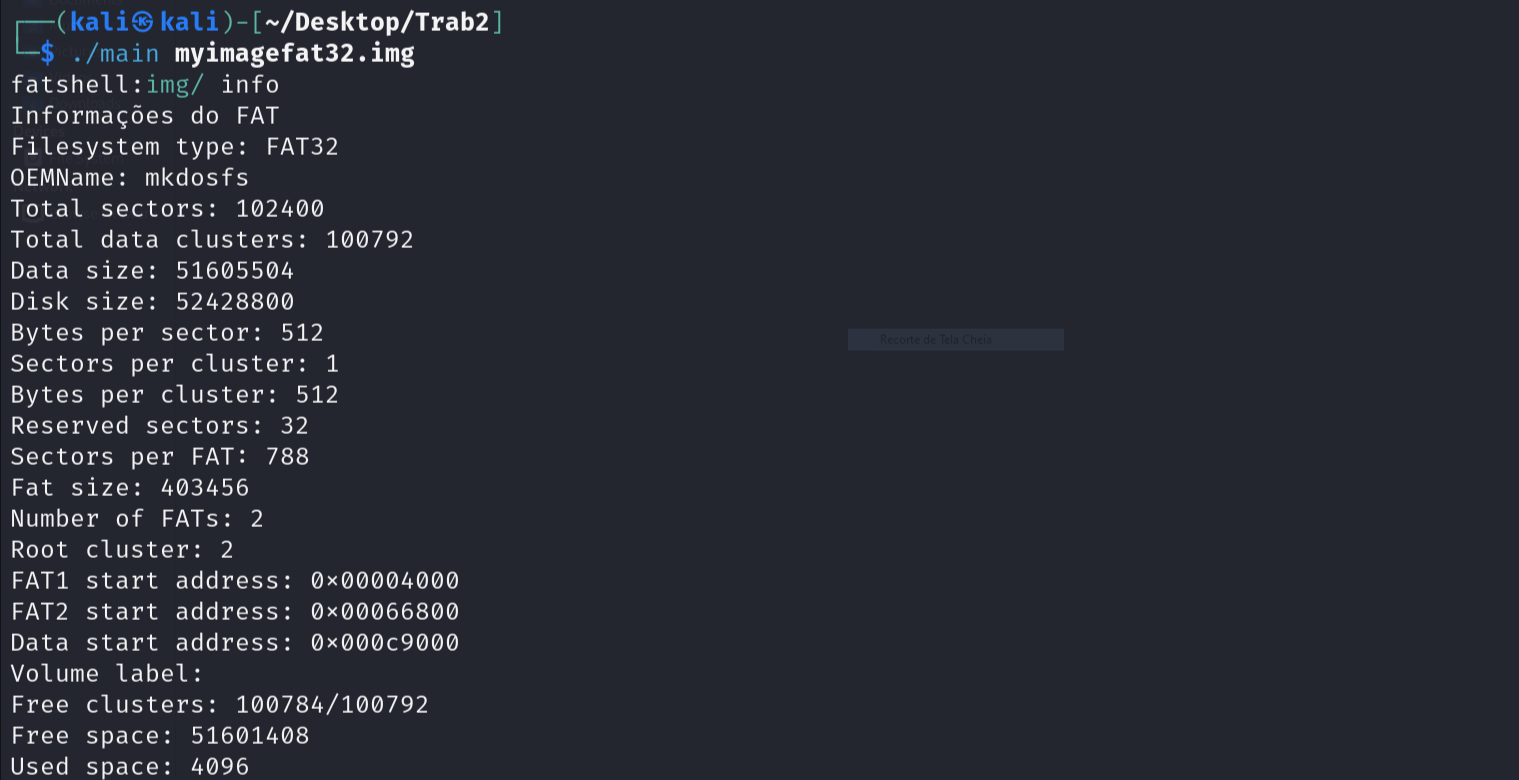
\includegraphics[width=450pt]{0-info.PNG}
    \caption{Saída do comando \texttt{info}}
    \label{fig:info}
\end{figure}

% --------------

\subsection{\texttt{ls}}
\label{subsec:ls}
Comando: \$ \texttt{ls [caminho]} 

O comando \texttt{ls} lista os arquivos e diretórios do caminho atual ou do caminho descrito no primeiro parâmetro dele, a sua saída executada no caminho atual pode ser verificada na Figura~\ref{fig:ls}.

\begin{figure}[H]
    \centering
    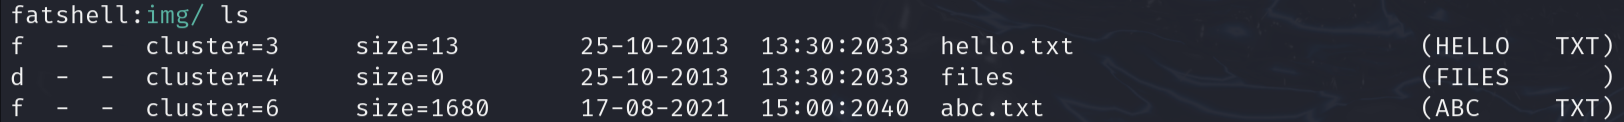
\includegraphics[width=450pt]{figuras/resultados/1-ls.PNG}
    \caption{Saída do comando \texttt{ls} executado no caminho atual}
    \label{fig:ls}
\end{figure}

% --------------

\subsection{\texttt{cluster}}
\label{subsec:cluster}
Comando: \$ \texttt{cluster <número do cluster>}

O comando \texttt{cluster} exibe o conteúdo de um cluster em específico, exemplo de uso na Figura~\ref{fig:cluester}.

\begin{figure}[H]
    \centering
    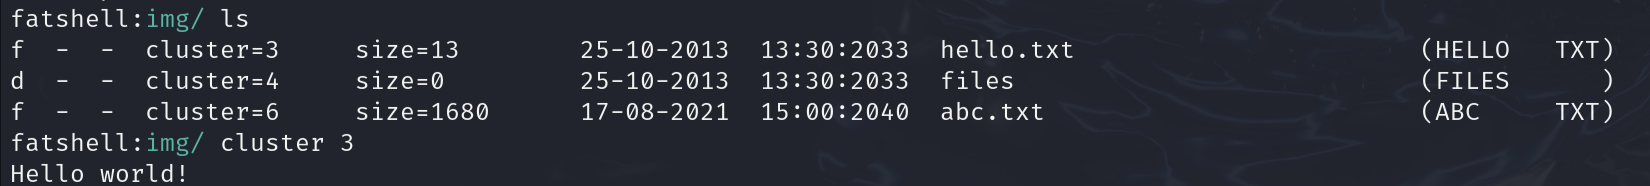
\includegraphics[width=450pt]{figuras/resultados/2-cluster.PNG}
    \caption{Saída do comando \texttt{cluster}}
    \label{fig:cluester}
\end{figure}

% --------------

\subsection{\texttt{cp}}
\label{subsec:cp}
Comando: \$ \texttt{cp <origem> <destino>}  

O comando \texttt{cp} realiza a cópia de um arquivo do caminho de origem para o caminho de destino, podendo efetuar a cópia entre o sistema da imagem e o sistema de arquivo do host sistemas de arquivos ou no próprio sistema da imagem. A cópia de um arquivo externo para o FAT32 pode ser verificada na Figura~\ref{fig:cp-externo-interno-1} e seu resultado na Figura~\ref{fig:cp-externo-interno-2}.

\begin{figure}[H]
    \centering
    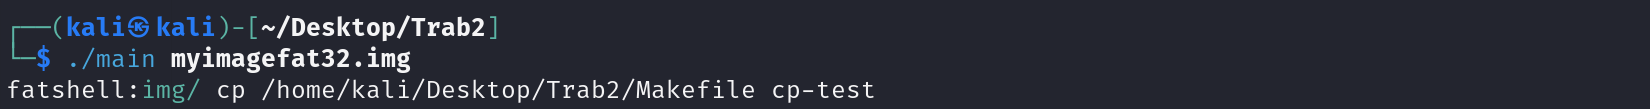
\includegraphics[width=450pt]{figuras/resultados/3.1-cp-externo-interno.PNG}
    \caption{Execução do comando \texttt{cp} para copiar arquivo externo para o FAT32}
    \label{fig:cp-externo-interno-1}
\end{figure}

\begin{figure}[H]
    \centering
    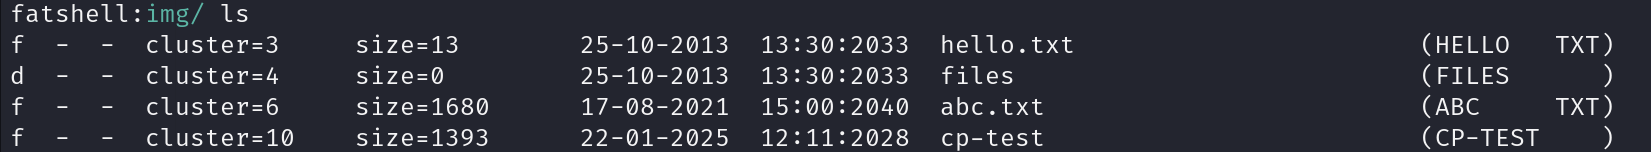
\includegraphics[width=450pt]{figuras/resultados/3.2-cp-externo-interno.PNG}
    \caption{Resultado da cópia do arquivo externo}
    \label{fig:cp-externo-interno-2}
\end{figure}

A cópia de um arquivo para o próprio FAT32 pode ser verificada na Figura~\ref{fig:cp-interno-attr}.

\begin{figure}[H]
    \centering
    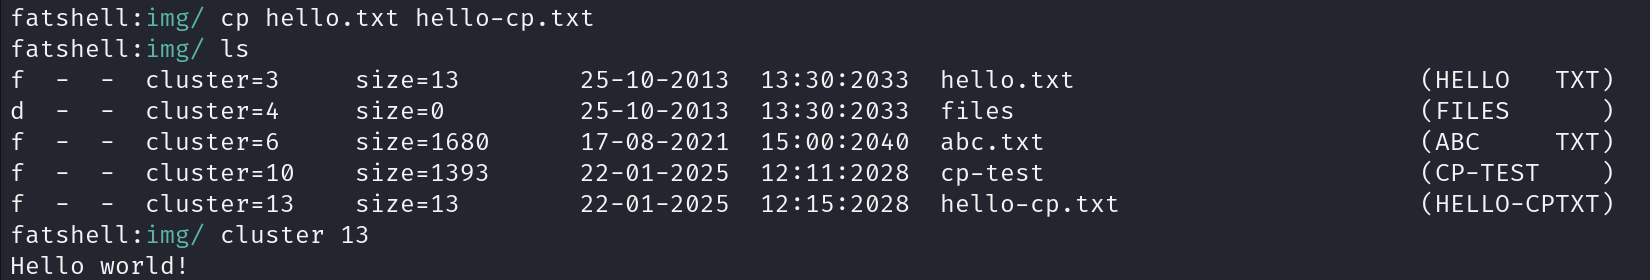
\includegraphics[width=450pt]{figuras/resultados/5-cp-interno-attr.PNG}
    \caption{Execução e resultado do comando \texttt{cp}, utilizado no próprio FAT32}
    \label{fig:cp-interno-attr}
\end{figure}

A cópia do arquivo residente no FAT32 para o sistema de arquivos externo pode ser verificada na Figura~\ref{fig:cp-interno-externo-1} e o seu resultado na Figura~\ref{fig:cp-interno-externo-2}.

\begin{figure}[H]
    \centering
    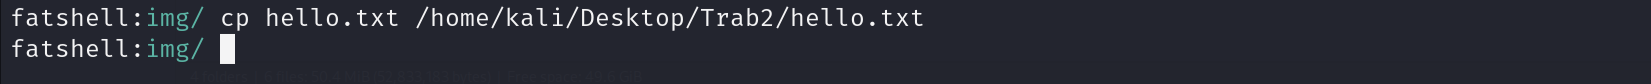
\includegraphics[width=450pt]{figuras/resultados/6-cp-interno-externo.PNG}
    \caption{Execução do comando \texttt{cp} realizando a cópia de um arquivo interno para o sistema de arquivos externo}
    \label{fig:cp-interno-externo-1}
\end{figure}

\begin{figure}[H]
    \centering
    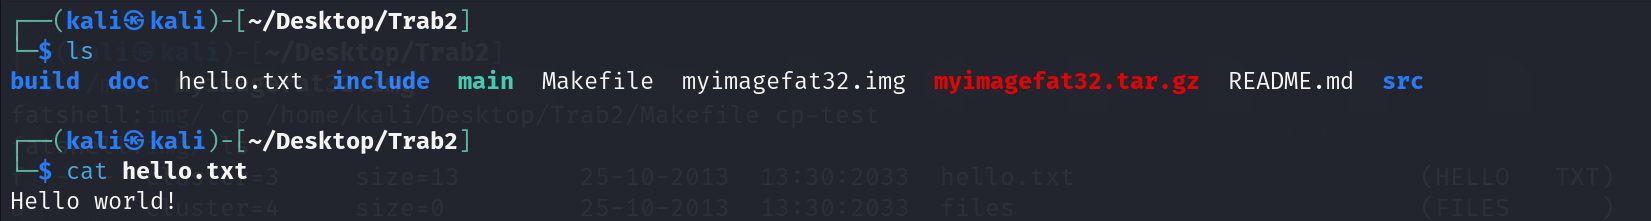
\includegraphics[width=450pt]{figuras/resultados/7-cp-arquivo-externo-resultado.PNG}
    \caption{Resultado no sistema de arquivos internos após cópia de arquivo resistente no FAT32}
    \label{fig:cp-interno-externo-2}
\end{figure}

% --------------

\subsection{\texttt{attr}}
\label{subsec:attr}
Comando: \$ \texttt{attr <diretório | arquivo> }

O comando \texttt{attr} exibe os atributos de um arquivo ou diretório, a Figura~\ref{fig:attr} mostra a saída deste comando.

\begin{figure}[H]
    \centering
    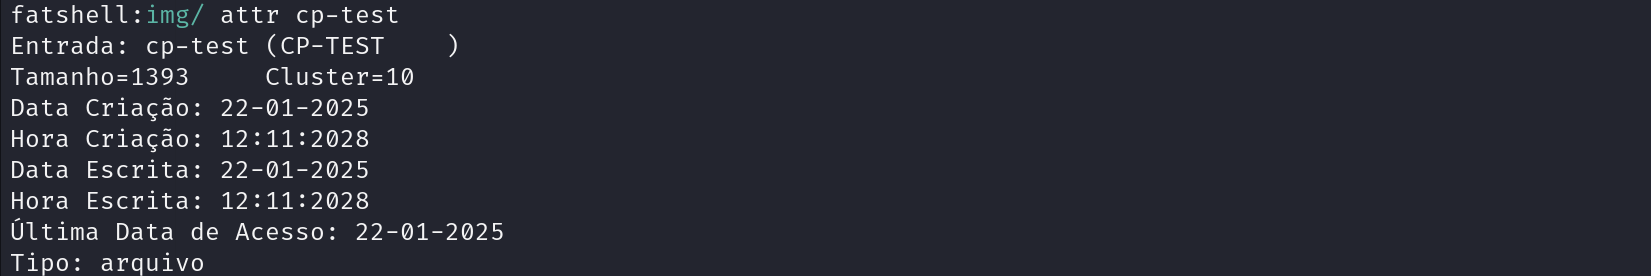
\includegraphics[width=450pt]{figuras/resultados/4-attr.PNG}
    \caption{Exemplo de saída para o comando \texttt{attr} utilizado em um arquivo}
    \label{fig:attr}
\end{figure}

% --------------

\subsection{\texttt{touch}}
\label{subsec:touch}
Comando: \$ \texttt{touch <nome>} 

O comando \texttt{touch} cria um arquivo sem conteúdo, a Figura~\ref{fig:touch} mostra a execução deste comando.

\begin{figure}[h!]
    \centering
    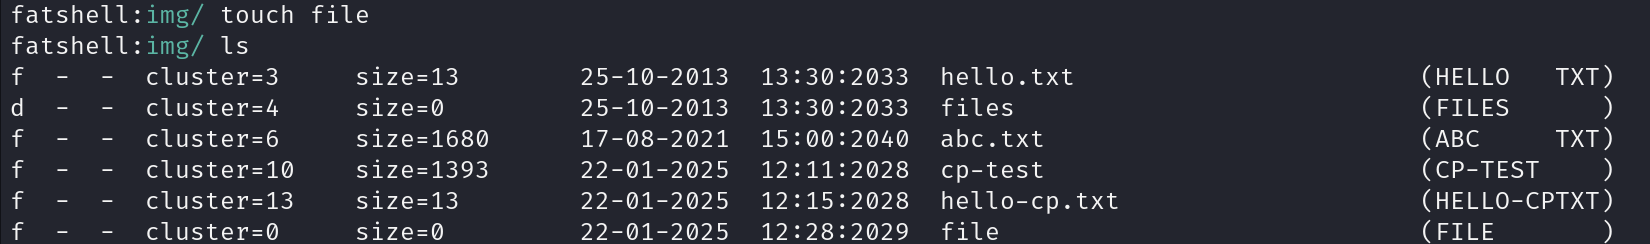
\includegraphics[width=450pt]{figuras/resultados/8-touch.PNG}
    \caption{Exemplo de uso do comando \texttt{touch}}
    \label{fig:touch}
\end{figure}

% --------------

\subsection{\texttt{mkdir}}
\label{subsec:mkdir}
Comando: \$ \texttt{mkdir <nome>}

O comando \texttt{mkdir} cria um diretório vazio, um exemplo da sua utilização pode ser analisado na Figura~\ref{fig:mkdir}.

\begin{figure}[H]
    \centering
    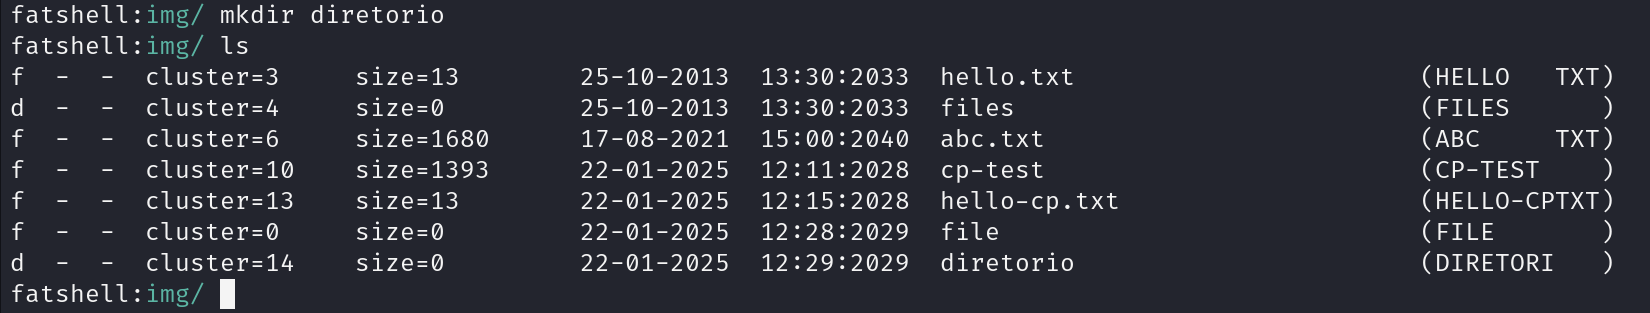
\includegraphics[width=450pt]{figuras/resultados/9-mkdir.PNG}
    \caption{Exemplo de uso do comando \texttt{mkdir}}
    \label{fig:mkdir}
\end{figure}

% --------------

\subsection{\texttt{cd}}
\label{subsec:cd}
Comando: \$ \texttt{cd <destino>}

O comando \texttt{cd} possibilita navegar entre os diretórios, um exemplo da sua utilização pode ser analisado na Figura~\ref{fig:cd}.
 
\begin{figure}[H]
    \centering
    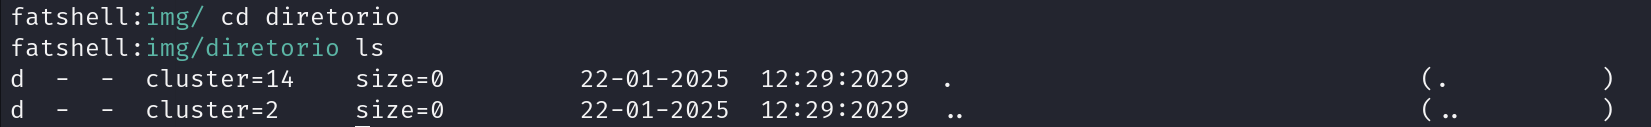
\includegraphics[width=450pt]{figuras/resultados/10-cd.PNG}
    \caption{Exemplo de utilização do comando \texttt{cd}}
    \label{fig:cd}
\end{figure}

% --------------

\subsection{\texttt{rename}}
\label{subsec:rename}
Comando: \$ \texttt{rename <arquivo alvo> <arquivo com novo nome>}

O comando \texttt{rename} altera o nome de um arquivo específico, um exemplo da sua utilização pode ser analisado na Figura~\ref{fig:rename}.

\begin{figure}[H]
    \centering
    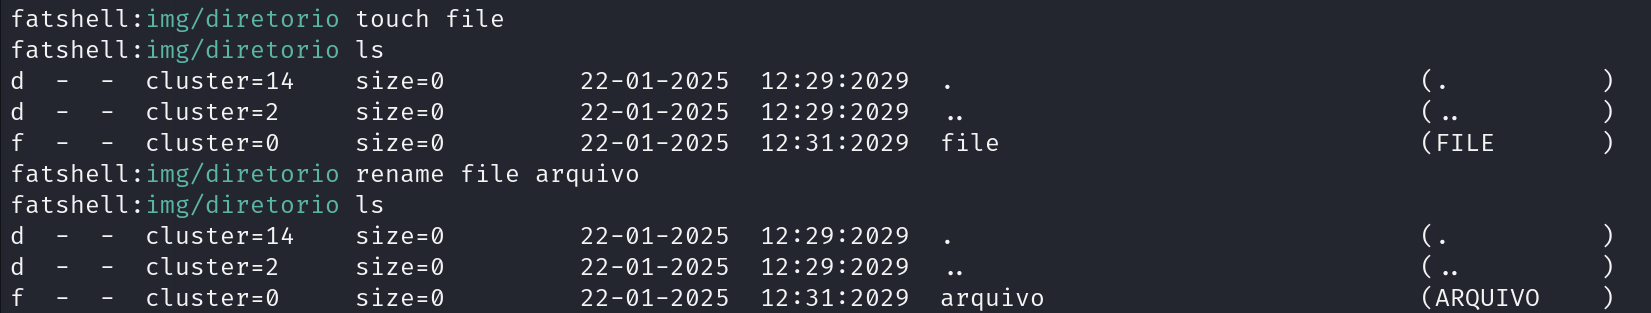
\includegraphics[width=450pt]{figuras/resultados/11-rename.PNG}
    \caption{Exemplo de utilização do comando \texttt{rename}}
    \label{fig:rename}
\end{figure}

% --------------

\subsection{\texttt{mv}}
\label{subsec:mv}
Comando: \$ \texttt{mv <origem> <destino>}

O comando \texttt{mv} move arquivos para um destino específico, assim como o comando \texttt{cp} também pode ser usado para interagir com o sistema de arquivo original do sistema operacional, um exemplo da sua utilização movendo um arquivo do sistema de arquivos externo para o FAT32, pode ser analisado na Figura~\ref{subsec:mv}.

\begin{figure}[H]
    \centering
    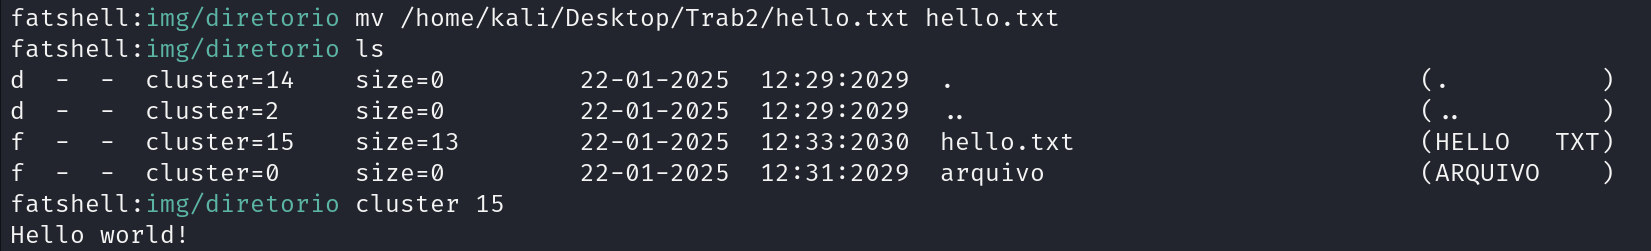
\includegraphics[width=450pt]{figuras/resultados/12-mv-externo-iterno.PNG}
    \caption{Exemplo do comando \texttt{mv} movendo arquivo externo para o FAT32}
    \label{fig:mv-externo-interno}
\end{figure}

O exemplo de mover um arquivo do FAT32 para o sistema de arquivos externo pode ser analisado na Figura~\ref{fig:mv-interno-externo} e sua validação na Figura~\ref{fig:mv-externo-validacao}.

\begin{figure}[H]
    \centering
    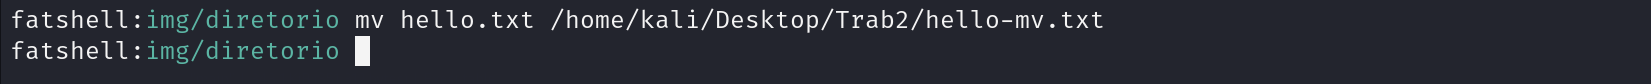
\includegraphics[width=450pt]{figuras/resultados/13-mv-interno-externo.PNG}
    \caption{Exemplo do comando \texttt{mv} movendo um arquivo do FAT32 para o sistema de arquivos externo}
    \label{fig:mv-interno-externo}
\end{figure}

\begin{figure}[H]
    \centering
    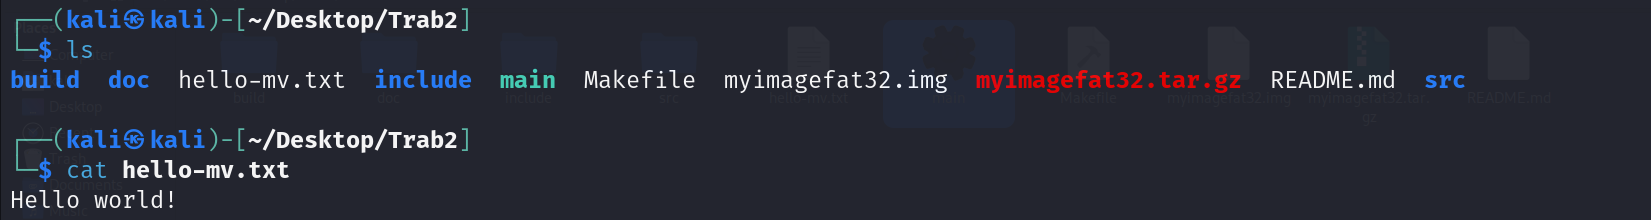
\includegraphics[width=450pt]{figuras/resultados/14-mv-externo-validacao.PNG}
    \caption{Resultado do comando \texttt{mv} movendo um arquivo do FAT32 para o sistema de arquivos externo}
    \label{fig:mv-externo-validacao}
\end{figure}

O exemplo de mover um arquivo interno para o próprio FAT32, pode ser verificado na Figura~\ref{fig:mv-interno}.

\begin{figure}[H]
    \centering
    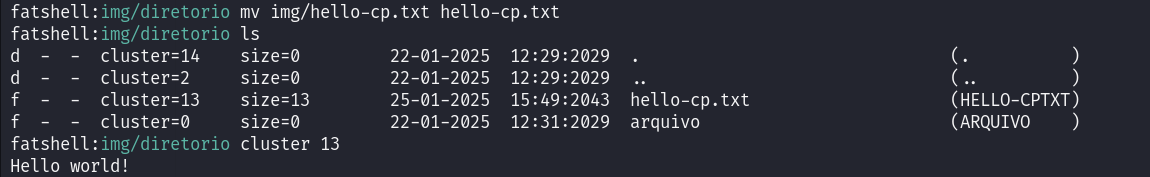
\includegraphics[width=450pt]{figuras/resultados/18-mv-interno-interno.PNG}
    \caption{Exemplo do comando \texttt{mv} movendo arquivo internamente no FAT32}
    \label{fig:mv-interno}
\end{figure}

% --------------

\subsection{\texttt{rm}}
\label{subsec:rm}
Comando: \$ \texttt{rm <arquivo>}

O comando \texttt{rm} remove um arquivo em específico do sistema de arquivos, um exemplo para sua utilização pode ser encontrado na Figura~\ref{fig:rm}.

\begin{figure}[H]
    \centering
    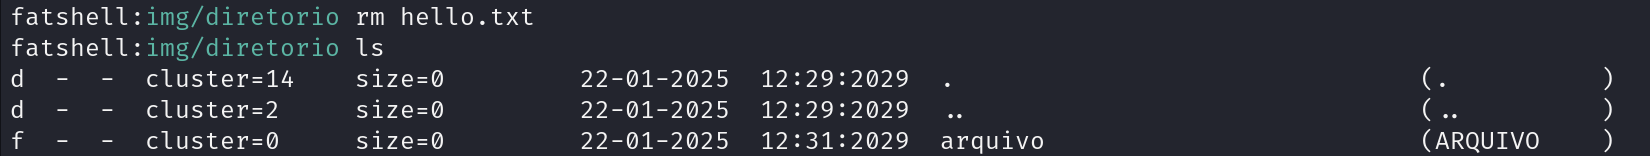
\includegraphics[width=450pt]{figuras/resultados/16-rm.PNG}
    \caption{Exemplo da utilização do comando \texttt{rm}}
    \label{fig:rm}
\end{figure}

% --------------

\subsection{\texttt{rmdir}}
\label{subsec:rmdir}
Comando: \$ \texttt{rmdir <diretório>}

O comando \texttt{rmdir} remove um diretório específico caso ele esteja vazio, um exemplo da sua utilização pode ser encontrado na Figura~\ref{fig:rmdir}.

\begin{figure}[H]
    \centering
    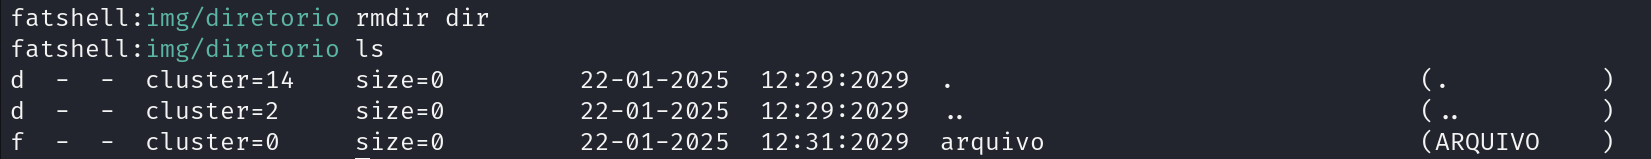
\includegraphics[width=450pt]{figuras/resultados/17-rmdir.PNG}
    \caption{Exemplo da utilização do comando \texttt{rmdir}}
    \label{fig:rmdir}
\end{figure}

% --------------

\subsection{\texttt{pwd}}
\label{subsec:pwd}
Comando: \$ \texttt{pwd}

O comando \texttt{pwd} exibe o caminho absoluto atual, um exemplo da sua saída pode ser encontrado na Figura~\ref{fig:pwd}.

\begin{figure}[H]
    \centering
    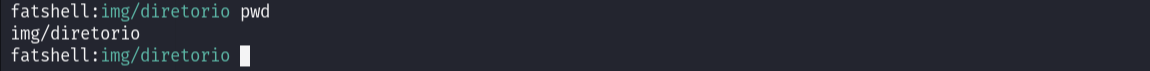
\includegraphics[width=450pt]{figuras/resultados/19-pwd.PNG}
    \caption{Exemplo da saída do comando \texttt{pwd}}
    \label{fig:pwd}
\end{figure}

% --------------

\section{Conclusões}
\label{sec:conclusoes}
A implementação do sistema de arquivos FAT32 permitiu consolidar conceitos teóricos sobre a organização e implementação de um sistema de arquivos, em especial o FAT32, destacando a sua organização de dados em disco, gerenciamento de metadados e alocação de clusters. A estrutura modular do código, dividida em componentes como tabela FAT, entradas de diretório e manipulação de imagens de disco, facilitou a manutenção e o teste individual de cada funcionalidade. O \textit{shell} desenvolvido provou ser eficaz na interação com o sistema, executando comandos complexos como cópia entre sistemas de arquivos externos e internos, movimentação de arquivos e renomeação. Os principais desafios durante a implementação do sistema foi a manipulação de nomes longos e a garantia de integridade do sistema todo. Ainda assim, acreditamos que o resultado foi positivo, tanto para o nosso aprendizado quanto para o êxito do projeto em si.

% ----------------------------------------------------------
% ELEMENTOS PÓS-TEXTUAIS
% ----------------------------------------------------------
\postextual
% ----------------------------------------------------------
% Referências bibliográficas
% ----------------------------------------------------------
\renewcommand{\bibsection}{%
\section{\bibname}
\bibmark
%\ifnobibintoc\else
%\phantomsection
%\addcontentsline{toc}{section}{\bibname}
%\fi
\prebibhook}

\bibliography{abntex2-modelo-references}

\end{document}
